\documentclass[a4paper]{book}
\usepackage{a4wide}
\usepackage{makeidx}
\usepackage{fancyhdr}
\usepackage{graphicx}
\usepackage{multicol}
\usepackage{float}
\usepackage{textcomp}
\usepackage{alltt}
\usepackage{times}
\usepackage{ifpdf}
\ifpdf
\usepackage[pdftex,
            pagebackref=true,
            colorlinks=true,
            linkcolor=blue,
            unicode
           ]{hyperref}
\else
\usepackage[ps2pdf,
            pagebackref=true,
            colorlinks=true,
            linkcolor=blue,
            unicode
           ]{hyperref}
\usepackage{pspicture}
\fi
\usepackage[utf8]{inputenc}
\usepackage{doxygen}
\makeindex
\setcounter{tocdepth}{3}
\renewcommand{\footrulewidth}{0.4pt}
\begin{document}
\begin{titlepage}
\vspace*{7cm}
\begin{center}
{\Large Monde des cubes \\[1ex]\large 0.1 }\\
\vspace*{1cm}
{\large Generated by Doxygen 1.5.7.1}\\
\vspace*{0.5cm}
{\small Thu May 7 22:38:32 2009}\\
\end{center}
\end{titlepage}
\clearemptydoublepage
\pagenumbering{roman}
\tableofcontents
\clearemptydoublepage
\pagenumbering{arabic}
\chapter{Class Index}
\section{Class Hierarchy}
This inheritance list is sorted roughly, but not completely, alphabetically:\begin{CompactList}
\item \contentsline{section}{EcoAgent}{\pageref{classEcoAgent}}{}
\begin{CompactList}
\item \contentsline{section}{Cube}{\pageref{classCube}}{}
\item \contentsline{section}{Table}{\pageref{classTable}}{}
\end{CompactList}
\item \contentsline{section}{EcoAgentID}{\pageref{classEcoAgentID}}{}
\item \contentsline{section}{PlateformeEcoResolution}{\pageref{classPlateformeEcoResolution}}{}
\begin{CompactList}
\item \contentsline{section}{PlateformeMondeDesCubes}{\pageref{classPlateformeMondeDesCubes}}{}
\end{CompactList}
\item \contentsline{section}{Regle}{\pageref{classRegle}}{}
\item \contentsline{section}{Singleton$<$ T $>$}{\pageref{classSingleton}}{}
\item \contentsline{section}{Singleton$<$ PlateformeMondeDesCubes $>$}{\pageref{classSingleton}}{}
\begin{CompactList}
\item \contentsline{section}{PlateformeMondeDesCubes}{\pageref{classPlateformeMondeDesCubes}}{}
\end{CompactList}
\end{CompactList}

\chapter{Class Index}
\section{Class List}
Here are the classes, structs, unions and interfaces with brief descriptions:\begin{CompactList}
\item\contentsline{section}{\hyperlink{classEcoAgent}{EcoAgent} (Classe abstraite appelee par les classes Cube et Table )}{\pageref{classEcoAgent}}{}
\item\contentsline{section}{\hyperlink{classPlateformeEcoResolution}{PlateformeEcoResolution} (Classe representant une plateforme d'eco-resolution abstraite )}{\pageref{classPlateformeEcoResolution}}{}
\item\contentsline{section}{\hyperlink{classSingleton}{Singleton$<$ T $>$} (Template de classe permettant de rendre une classe instanciable une seule fois )}{\pageref{classSingleton}}{}
\end{CompactList}

\chapter{File Index}
\section{File List}
Here is a list of all documented files with brief descriptions:\begin{CompactList}
\item\contentsline{section}{trunk/include/\hyperlink{cube_8hpp}{cube.hpp} (Implementation du module cube qui est un derive d'un \hyperlink{classEcoAgent}{EcoAgent} )}{\pageref{cube_8hpp}}{}
\item\contentsline{section}{trunk/include/\hyperlink{ecoAgent_8hpp}{ecoAgent.hpp} (Mise en place de la classe abstraite \hyperlink{classEcoAgent}{EcoAgent} )}{\pageref{ecoAgent_8hpp}}{}
\item\contentsline{section}{trunk/include/\hyperlink{ecoAgentID_8hpp}{ecoAgentID.hpp} (Implementation de la classe \hyperlink{classEcoAgentID}{EcoAgentID} )}{\pageref{ecoAgentID_8hpp}}{}
\item\contentsline{section}{trunk/include/\hyperlink{etat_8hpp}{etat.hpp} (Enumeration des etats possibles des eco-agents )}{\pageref{etat_8hpp}}{}
\item\contentsline{section}{trunk/include/\hyperlink{plateformeEcoResolution_8hpp}{plateformeEcoResolution.hpp} (Plateforme abstraite d'eco-resolution )}{\pageref{plateformeEcoResolution_8hpp}}{}
\item\contentsline{section}{trunk/include/\hyperlink{plateformeMondeDesCubes_8hpp}{plateformeMondeDesCubes.hpp} (Plateforme d'eco-resolution appliquee au monde des cubes )}{\pageref{plateformeMondeDesCubes_8hpp}}{}
\item\contentsline{section}{trunk/include/\hyperlink{regle_8hpp}{regle.hpp} (Squelette d'une regle pour une plateforme d'eco-resolution )}{\pageref{regle_8hpp}}{}
\item\contentsline{section}{trunk/include/\hyperlink{singleton_8hpp}{singleton.hpp} (Implementation du design pattern singleton )}{\pageref{singleton_8hpp}}{}
\item\contentsline{section}{trunk/include/\hyperlink{table_8hpp}{table.hpp} (Implementation du module table qui est un derive d'un \hyperlink{classEcoAgent}{EcoAgent} )}{\pageref{table_8hpp}}{}
\end{CompactList}

\chapter{Class Documentation}
\hypertarget{classAucuneSurcharge}{
\section{AucuneSurcharge Class Reference}
\label{classAucuneSurcharge}\index{AucuneSurcharge@{AucuneSurcharge}}
}
Cette classe contient les fonctions testant si les cubes ne portent pas plus de un cube.  


{\tt \#include $<$aucuneSurcharge.hpp$>$}

Inherits \hyperlink{classRegle}{Regle}.

Collaboration diagram for AucuneSurcharge:\subsection*{Public Member Functions}
\begin{CompactItemize}
\item 
\hypertarget{classAucuneSurcharge_691d3e7997769c020f40d708309f0f1d}{
void \hyperlink{classAucuneSurcharge_691d3e7997769c020f40d708309f0f1d}{initialiser} ()}
\label{classAucuneSurcharge_691d3e7997769c020f40d708309f0f1d}

\begin{CompactList}\small\item\em Suite d'operations realisees pour initialiser la regle. \item\end{CompactList}\item 
bool \hyperlink{classAucuneSurcharge_d96084db10b49f9c48f6cb005248f7c4}{verifier} ()
\begin{CompactList}\small\item\em Verification de la regle generale : pour l'ensemble des cubes, sont-ils et seront-ils surcharges? \item\end{CompactList}\item 
bool \hyperlink{classAucuneSurcharge_985f14cd31785475866dc1081a41e2e1}{pasSurcharges} ()
\begin{CompactList}\small\item\em Verification d'un element de la regle generale: les cubes sont-ils surcharges? \item\end{CompactList}\item 
bool \hyperlink{classAucuneSurcharge_a866df9a186c7b922890cf00af2b58e2}{serontPasSurcharges} ()
\begin{CompactList}\small\item\em Verification d'un element de la regle generale: les cubes seront-ils surcharges? \item\end{CompactList}\end{CompactItemize}


\subsection{Detailed Description}
Cette classe contient les fonctions testant si les cubes ne portent pas plus de un cube. 

\subsection{Member Function Documentation}
\hypertarget{classAucuneSurcharge_985f14cd31785475866dc1081a41e2e1}{
\index{AucuneSurcharge@{AucuneSurcharge}!pasSurcharges@{pasSurcharges}}
\index{pasSurcharges@{pasSurcharges}!AucuneSurcharge@{AucuneSurcharge}}
\subsubsection[{pasSurcharges}]{\setlength{\rightskip}{0pt plus 5cm}bool AucuneSurcharge::pasSurcharges ()}}
\label{classAucuneSurcharge_985f14cd31785475866dc1081a41e2e1}


Verification d'un element de la regle generale: les cubes sont-ils surcharges? 

\begin{Desc}
\item[Returns:]true si le cas est verifiee, false sinon \end{Desc}
\hypertarget{classAucuneSurcharge_a866df9a186c7b922890cf00af2b58e2}{
\index{AucuneSurcharge@{AucuneSurcharge}!serontPasSurcharges@{serontPasSurcharges}}
\index{serontPasSurcharges@{serontPasSurcharges}!AucuneSurcharge@{AucuneSurcharge}}
\subsubsection[{serontPasSurcharges}]{\setlength{\rightskip}{0pt plus 5cm}bool AucuneSurcharge::serontPasSurcharges ()}}
\label{classAucuneSurcharge_a866df9a186c7b922890cf00af2b58e2}


Verification d'un element de la regle generale: les cubes seront-ils surcharges? 

\begin{Desc}
\item[Returns:]true si le cas est verifiee, false sinon \end{Desc}
\hypertarget{classAucuneSurcharge_d96084db10b49f9c48f6cb005248f7c4}{
\index{AucuneSurcharge@{AucuneSurcharge}!verifier@{verifier}}
\index{verifier@{verifier}!AucuneSurcharge@{AucuneSurcharge}}
\subsubsection[{verifier}]{\setlength{\rightskip}{0pt plus 5cm}bool AucuneSurcharge::verifier ()\hspace{0.3cm}{\tt  \mbox{[}virtual\mbox{]}}}}
\label{classAucuneSurcharge_d96084db10b49f9c48f6cb005248f7c4}


Verification de la regle generale : pour l'ensemble des cubes, sont-ils et seront-ils surcharges? 

\begin{Desc}
\item[Returns:]true si la regle est verifiee, false sinon \end{Desc}


Implements \hyperlink{classRegle_4b3de9a64ec0e948e9177026afcc073d}{Regle}.

The documentation for this class was generated from the following files:\begin{CompactItemize}
\item 
trunk/include/\hyperlink{aucuneSurcharge_8hpp}{aucuneSurcharge.hpp}\item 
trunk/src/aucuneSurcharge.cpp\end{CompactItemize}

\hypertarget{structcompareEcoAgentID}{
\section{compareEcoAgentID Class Reference}
\label{structcompareEcoAgentID}\index{compareEcoAgentID@{compareEcoAgentID}}
}
Structure contenant la redefinition de l'operateur de comparaison d'EcoAgentID Structure contenant la redefinition de l'operateur de comparaison d'EcoAgentID pour le transformer en cle unique d'une map.  


{\tt \#include $<$compareEcoAgentID.hpp$>$}



\subsection{Detailed Description}
Structure contenant la redefinition de l'operateur de comparaison d'EcoAgentID Structure contenant la redefinition de l'operateur de comparaison d'EcoAgentID pour le transformer en cle unique d'une map. 

The documentation for this class was generated from the following file:\begin{CompactItemize}
\item 
trunk/include/\hyperlink{compareEcoAgentID_8hpp}{compareEcoAgentID.hpp}\end{CompactItemize}

\hypertarget{classCube}{
\section{Cube Class Reference}
\label{classCube}\index{Cube@{Cube}}
}
Classe derivee de la classe \hyperlink{classEcoAgent}{EcoAgent} designant un \hyperlink{classCube}{Cube}.  


{\tt \#include $<$cube.hpp$>$}

Inherits \hyperlink{classEcoAgent}{EcoAgent}.

Collaboration diagram for Cube:\subsection*{Public Member Functions}
\begin{CompactItemize}
\item 
\hyperlink{classCube_06f3d86fb63e3aad08623610aa3c17b4}{Cube} ()
\begin{CompactList}\small\item\em Constructeur. \item\end{CompactList}\item 
\hyperlink{classCube_4793068a114fd49b51233e8f81884189}{Cube} (const \hyperlink{classEcoAgentID}{EcoAgentID} \&id)
\begin{CompactList}\small\item\em Constructeur. \item\end{CompactList}\item 
\hyperlink{classCube_a814e979cecb8c451fdb332ded2cea1e}{$\sim$Cube} ()
\begin{CompactList}\small\item\em Destructeur. \item\end{CompactList}\item 
\hypertarget{classCube_c81ac3b8da58ba8463d72e3a0433bafa}{
void \hyperlink{classCube_c81ac3b8da58ba8463d72e3a0433bafa}{rechercherFuite} ()}
\label{classCube_c81ac3b8da58ba8463d72e3a0433bafa}

\begin{CompactList}\small\item\em Suite d'operations realisees par le cube lorsqu'il cherche a fuir. \item\end{CompactList}\item 
\hypertarget{classCube_10f69d54f313f48ac0c8468628ac6902}{
void \hyperlink{classCube_10f69d54f313f48ac0c8468628ac6902}{rechercherSatisfaction} ()}
\label{classCube_10f69d54f313f48ac0c8468628ac6902}

\begin{CompactList}\small\item\em Suite d'operations realisees par le cube lorsqu'il cherche a se satisfaire. \item\end{CompactList}\item 
void \hyperlink{classCube_2b9c63b545c13c95b9a7f44c3c5147ad}{agresser} (const \hyperlink{classCube}{Cube} \&a)
\begin{CompactList}\small\item\em Suite d'operations realisees lorsque le cube agresse un autre eco-agent. \item\end{CompactList}\item 
\hypertarget{classCube_a9af44bff02fb06ac5be83f4c041fe57}{
void \hyperlink{classCube_a9af44bff02fb06ac5be83f4c041fe57}{estAgresse} ()}
\label{classCube_a9af44bff02fb06ac5be83f4c041fe57}

\begin{CompactList}\small\item\em Suite d'operations realisees par le cube lorsqu'il est agressee. \item\end{CompactList}\item 
\hypertarget{classCube_ce1011f5a33ce211d5ca44e029f59224}{
void \hyperlink{classCube_ce1011f5a33ce211d5ca44e029f59224}{faireFuite} ()}
\label{classCube_ce1011f5a33ce211d5ca44e029f59224}

\begin{CompactList}\small\item\em Suite d'operations realisees par le cube lorsqu'il fuit. \item\end{CompactList}\item 
\hypertarget{classCube_1fec2199edab8e6cfdb3685256d2cdec}{
void \hyperlink{classCube_1fec2199edab8e6cfdb3685256d2cdec}{faireSatisfaction} ()}
\label{classCube_1fec2199edab8e6cfdb3685256d2cdec}

\begin{CompactList}\small\item\em Suite d'operations realisees par le cube lorsqu'il se satisfait. \item\end{CompactList}\item 
void \hyperlink{classCube_51dbc3cc9578d3cf5f9e56cab24aff1f}{initialiserEtat} ()
\begin{CompactList}\small\item\em Initialisation de l'etat du cube. \item\end{CompactList}\item 
\hypertarget{classCube_9289a4d72b849b7f868b189f531daa62}{
void \hyperlink{classCube_9289a4d72b849b7f868b189f531daa62}{agir} ()}
\label{classCube_9289a4d72b849b7f868b189f531daa62}

\begin{CompactList}\small\item\em Suite d'operations realisees par le cube lorsqu'il agit. \item\end{CompactList}\end{CompactItemize}


\subsection{Detailed Description}
Classe derivee de la classe \hyperlink{classEcoAgent}{EcoAgent} designant un \hyperlink{classCube}{Cube}. 

\subsection{Constructor \& Destructor Documentation}
\hypertarget{classCube_06f3d86fb63e3aad08623610aa3c17b4}{
\index{Cube@{Cube}!Cube@{Cube}}
\index{Cube@{Cube}!Cube@{Cube}}
\subsubsection[{Cube}]{\setlength{\rightskip}{0pt plus 5cm}Cube::Cube ()}}
\label{classCube_06f3d86fb63e3aad08623610aa3c17b4}


Constructeur. 

Constructeur de la classe \hyperlink{classCube}{Cube} par defaut. Le cube recevra un \hyperlink{classEcoAgentID}{EcoAgentID} automatiquement genere. \hypertarget{classCube_4793068a114fd49b51233e8f81884189}{
\index{Cube@{Cube}!Cube@{Cube}}
\index{Cube@{Cube}!Cube@{Cube}}
\subsubsection[{Cube}]{\setlength{\rightskip}{0pt plus 5cm}Cube::Cube (const {\bf EcoAgentID} \& {\em id})}}
\label{classCube_4793068a114fd49b51233e8f81884189}


Constructeur. 

Constructeur de la classe \hyperlink{classCube}{Cube} avec un \hyperlink{classEcoAgentID}{EcoAgentID} specifique

\begin{Desc}
\item[Parameters:]
\begin{description}
\item[{\em id}]: identifiant unique que l'agent se verra attribuer \end{description}
\end{Desc}
\hypertarget{classCube_a814e979cecb8c451fdb332ded2cea1e}{
\index{Cube@{Cube}!$\sim$Cube@{$\sim$Cube}}
\index{$\sim$Cube@{$\sim$Cube}!Cube@{Cube}}
\subsubsection[{$\sim$Cube}]{\setlength{\rightskip}{0pt plus 5cm}Cube::$\sim$Cube ()}}
\label{classCube_a814e979cecb8c451fdb332ded2cea1e}


Destructeur. 

Destructeur de la classe \hyperlink{classCube}{Cube} 

\subsection{Member Function Documentation}
\hypertarget{classCube_2b9c63b545c13c95b9a7f44c3c5147ad}{
\index{Cube@{Cube}!agresser@{agresser}}
\index{agresser@{agresser}!Cube@{Cube}}
\subsubsection[{agresser}]{\setlength{\rightskip}{0pt plus 5cm}void Cube::agresser (const {\bf Cube} \& {\em a})}}
\label{classCube_2b9c63b545c13c95b9a7f44c3c5147ad}


Suite d'operations realisees lorsque le cube agresse un autre eco-agent. 

\begin{Desc}
\item[Parameters:]
\begin{description}
\item[{\em a}]: \hyperlink{classEcoAgent}{EcoAgent} a agresser \end{description}
\end{Desc}
\hypertarget{classCube_51dbc3cc9578d3cf5f9e56cab24aff1f}{
\index{Cube@{Cube}!initialiserEtat@{initialiserEtat}}
\index{initialiserEtat@{initialiserEtat}!Cube@{Cube}}
\subsubsection[{initialiserEtat}]{\setlength{\rightskip}{0pt plus 5cm}void Cube::initialiserEtat ()}}
\label{classCube_51dbc3cc9578d3cf5f9e56cab24aff1f}


Initialisation de l'etat du cube. 

Cette methode permet d'initialiser l'etat du cube en prenant en compte sa position courante et sa position finale. Par exemple, si la position courante correspond a la position finale, cette methode initialisera l'Etat a \char`\"{}satisfait\char`\"{} 

The documentation for this class was generated from the following file:\begin{CompactItemize}
\item 
trunk/include/\hyperlink{cube_8hpp}{cube.hpp}\end{CompactItemize}

\hypertarget{classEcoAgent}{
\section{EcoAgent Class Reference}
\label{classEcoAgent}\index{EcoAgent@{EcoAgent}}
}
Classe abstraite appelee par les classes Cube et Table.  


{\tt \#include $<$ecoAgent.hpp$>$}



\subsection{Detailed Description}
Classe abstraite appelee par les classes Cube et Table. 

The documentation for this class was generated from the following file:\begin{CompactItemize}
\item 
include/\hyperlink{ecoAgent_8hpp}{ecoAgent.hpp}\end{CompactItemize}

\hypertarget{classEcoAgentID}{
\section{EcoAgentID Class Reference}
\label{classEcoAgentID}\index{EcoAgentID@{EcoAgentID}}
}
Identifiant unique d'un eco-agent.  


{\tt \#include $<$ecoAgentID.hpp$>$}

\subsection*{Public Member Functions}
\begin{CompactItemize}
\item 
\hyperlink{classEcoAgentID_9c337e2ad56912db99193c03d1f82c56}{EcoAgentID} ()
\begin{CompactList}\small\item\em Constructeur. \item\end{CompactList}\item 
\hyperlink{classEcoAgentID_97da1c0ae8891bbf10feb0574ef64a26}{$\sim$EcoAgentID} ()
\begin{CompactList}\small\item\em Destructeur. \item\end{CompactList}\item 
int \hyperlink{classEcoAgentID_30abc8a92bd07523b8e4f4baf312b56e}{getId} () const 
\begin{CompactList}\small\item\em Obtention de l'identifiant. \item\end{CompactList}\item 
bool \hyperlink{classEcoAgentID_a6c183361e0ccdab9da2c6666d77c111}{operator==} (const \hyperlink{classEcoAgentID}{EcoAgentID} \&) const 
\begin{CompactList}\small\item\em Comparaison de \hyperlink{classEcoAgentID}{EcoAgentID}. \item\end{CompactList}\item 
bool \hyperlink{classEcoAgentID_24d44b31302cd2761ffce1df8f74f12c}{operator$<$} (const \hyperlink{classEcoAgentID}{EcoAgentID} \&) const 
\begin{CompactList}\small\item\em Comparaison de \hyperlink{classEcoAgentID}{EcoAgentID}. \item\end{CompactList}\end{CompactItemize}
\subsection*{Static Public Member Functions}
\begin{CompactItemize}
\item 
\hypertarget{classEcoAgentID_9b8f29915bff7e36bf53e695c148517e}{
static int \hyperlink{classEcoAgentID_9b8f29915bff7e36bf53e695c148517e}{getNombreDeGeneration} ()}
\label{classEcoAgentID_9b8f29915bff7e36bf53e695c148517e}

\begin{CompactList}\small\item\em Obtention du nombre de generation Methode statique qui permet d'obtenir le nombre de generations d'EcoAgentID. \item\end{CompactList}\end{CompactItemize}


\subsection{Detailed Description}
Identifiant unique d'un eco-agent. 

La classe \hyperlink{classEcoAgentID}{EcoAgentID} represente un identifiant unique d'un eco-agent. Il permet la generation automatique des identifiants 

\subsection{Constructor \& Destructor Documentation}
\hypertarget{classEcoAgentID_9c337e2ad56912db99193c03d1f82c56}{
\index{EcoAgentID@{EcoAgentID}!EcoAgentID@{EcoAgentID}}
\index{EcoAgentID@{EcoAgentID}!EcoAgentID@{EcoAgentID}}
\subsubsection[{EcoAgentID}]{\setlength{\rightskip}{0pt plus 5cm}EcoAgentID::EcoAgentID ()}}
\label{classEcoAgentID_9c337e2ad56912db99193c03d1f82c56}


Constructeur. 

Constructeur de la classe \hyperlink{classEcoAgentID}{EcoAgentID} \hypertarget{classEcoAgentID_97da1c0ae8891bbf10feb0574ef64a26}{
\index{EcoAgentID@{EcoAgentID}!$\sim$EcoAgentID@{$\sim$EcoAgentID}}
\index{$\sim$EcoAgentID@{$\sim$EcoAgentID}!EcoAgentID@{EcoAgentID}}
\subsubsection[{$\sim$EcoAgentID}]{\setlength{\rightskip}{0pt plus 5cm}EcoAgentID::$\sim$EcoAgentID ()}}
\label{classEcoAgentID_97da1c0ae8891bbf10feb0574ef64a26}


Destructeur. 

Destructeur de la classe \hyperlink{classEcoAgentID}{EcoAgentID} 

\subsection{Member Function Documentation}
\hypertarget{classEcoAgentID_30abc8a92bd07523b8e4f4baf312b56e}{
\index{EcoAgentID@{EcoAgentID}!getId@{getId}}
\index{getId@{getId}!EcoAgentID@{EcoAgentID}}
\subsubsection[{getId}]{\setlength{\rightskip}{0pt plus 5cm}int EcoAgentID::getId () const}}
\label{classEcoAgentID_30abc8a92bd07523b8e4f4baf312b56e}


Obtention de l'identifiant. 

Methode qui retourne l'identifiant de l'eco-agent \hypertarget{classEcoAgentID_24d44b31302cd2761ffce1df8f74f12c}{
\index{EcoAgentID@{EcoAgentID}!operator$<$@{operator$<$}}
\index{operator$<$@{operator$<$}!EcoAgentID@{EcoAgentID}}
\subsubsection[{operator$<$}]{\setlength{\rightskip}{0pt plus 5cm}bool EcoAgentID::operator$<$ (const {\bf EcoAgentID} \& {\em eid}) const}}
\label{classEcoAgentID_24d44b31302cd2761ffce1df8f74f12c}


Comparaison de \hyperlink{classEcoAgentID}{EcoAgentID}. 

Methode qui permet de comparer deux \hyperlink{classEcoAgentID}{EcoAgentID} \hypertarget{classEcoAgentID_a6c183361e0ccdab9da2c6666d77c111}{
\index{EcoAgentID@{EcoAgentID}!operator==@{operator==}}
\index{operator==@{operator==}!EcoAgentID@{EcoAgentID}}
\subsubsection[{operator==}]{\setlength{\rightskip}{0pt plus 5cm}bool EcoAgentID::operator== (const {\bf EcoAgentID} \& {\em eid}) const}}
\label{classEcoAgentID_a6c183361e0ccdab9da2c6666d77c111}


Comparaison de \hyperlink{classEcoAgentID}{EcoAgentID}. 

Methode qui permet de comparer deux \hyperlink{classEcoAgentID}{EcoAgentID} 

The documentation for this class was generated from the following files:\begin{CompactItemize}
\item 
trunk/include/\hyperlink{ecoAgentID_8hpp}{ecoAgentID.hpp}\item 
trunk/src/ecoAgent.cpp\end{CompactItemize}

\hypertarget{classExceptionCubeNonRelie}{
\section{ExceptionCubeNonRelie Class Reference}
\label{classExceptionCubeNonRelie}\index{ExceptionCubeNonRelie@{ExceptionCubeNonRelie}}
}
Exception lancee dans le cadre de la verification de la regle \char`\"{}est-ce que les cubes sont relies a la table\char`\"{}.  


{\tt \#include $<$Exceptions.hpp$>$}



\subsection{Detailed Description}
Exception lancee dans le cadre de la verification de la regle \char`\"{}est-ce que les cubes sont relies a la table\char`\"{}. 

The documentation for this class was generated from the following file:\begin{CompactItemize}
\item 
trunk/include/\hyperlink{Exceptions_8hpp}{Exceptions.hpp}\end{CompactItemize}

\hypertarget{classExceptionCubeSeraNonRelie}{
\section{ExceptionCubeSeraNonRelie Class Reference}
\label{classExceptionCubeSeraNonRelie}\index{ExceptionCubeSeraNonRelie@{ExceptionCubeSeraNonRelie}}
}
Exception lancee dans le cadre de la verification de la regle \char`\"{}est-ce que les cubes seront relies a la table\char`\"{}.  


{\tt \#include $<$Exceptions.hpp$>$}



\subsection{Detailed Description}
Exception lancee dans le cadre de la verification de la regle \char`\"{}est-ce que les cubes seront relies a la table\char`\"{}. 

The documentation for this class was generated from the following file:\begin{CompactItemize}
\item 
trunk/include/\hyperlink{Exceptions_8hpp}{Exceptions.hpp}\end{CompactItemize}

\hypertarget{classExceptionEcoAgentDejaEnregistre}{
\section{ExceptionEcoAgentDejaEnregistre Class Reference}
\label{classExceptionEcoAgentDejaEnregistre}\index{ExceptionEcoAgentDejaEnregistre@{ExceptionEcoAgentDejaEnregistre}}
}
Exception lancee dans le cadre de l'ajout d'un \hyperlink{classEcoAgent}{EcoAgent} deja enregistre dans une \hyperlink{classPlateformeEcoResolution}{PlateformeEcoResolution}.  


{\tt \#include $<$ExceptionEcoAgentDejaEnregistre.hpp$>$}



\subsection{Detailed Description}
Exception lancee dans le cadre de l'ajout d'un \hyperlink{classEcoAgent}{EcoAgent} deja enregistre dans une \hyperlink{classPlateformeEcoResolution}{PlateformeEcoResolution}. 

The documentation for this class was generated from the following file:\begin{CompactItemize}
\item 
trunk/include/\hyperlink{ExceptionEcoAgentDejaEnregistre_8hpp}{ExceptionEcoAgentDejaEnregistre.hpp}\end{CompactItemize}

\hypertarget{classExceptionIlExisteraUneBoucle}{
\section{ExceptionIlExisteraUneBoucle Class Reference}
\label{classExceptionIlExisteraUneBoucle}\index{ExceptionIlExisteraUneBoucle@{ExceptionIlExisteraUneBoucle}}
}
Exception lancee dans le cadre de la verification de la regle \char`\"{}est-ce que les cubes seront relies a la table\char`\"{}.  


{\tt \#include $<$Exceptions.hpp$>$}



\subsection{Detailed Description}
Exception lancee dans le cadre de la verification de la regle \char`\"{}est-ce que les cubes seront relies a la table\char`\"{}. 

The documentation for this class was generated from the following file:\begin{CompactItemize}
\item 
trunk/include/\hyperlink{Exceptions_8hpp}{Exceptions.hpp}\end{CompactItemize}

\hypertarget{classExceptionIlExisteUneBoucle}{
\section{ExceptionIlExisteUneBoucle Class Reference}
\label{classExceptionIlExisteUneBoucle}\index{ExceptionIlExisteUneBoucle@{ExceptionIlExisteUneBoucle}}
}
Exception lancee dans le cadre de la verification de la regle \char`\"{}est-ce que les cubes sont relies a la table\char`\"{}.  


{\tt \#include $<$Exceptions.hpp$>$}



\subsection{Detailed Description}
Exception lancee dans le cadre de la verification de la regle \char`\"{}est-ce que les cubes sont relies a la table\char`\"{}. 

The documentation for this class was generated from the following file:\begin{CompactItemize}
\item 
trunk/include/\hyperlink{Exceptions_8hpp}{Exceptions.hpp}\end{CompactItemize}

\hypertarget{classExceptionUnCubeEstSurcharge}{
\section{ExceptionUnCubeEstSurcharge Class Reference}
\label{classExceptionUnCubeEstSurcharge}\index{ExceptionUnCubeEstSurcharge@{ExceptionUnCubeEstSurcharge}}
}
Exception lancee dans le cadre de la verification de la regle \char`\"{}est-ce que les cubes sont surcharges\char`\"{}.  


{\tt \#include $<$Exceptions.hpp$>$}



\subsection{Detailed Description}
Exception lancee dans le cadre de la verification de la regle \char`\"{}est-ce que les cubes sont surcharges\char`\"{}. 

The documentation for this class was generated from the following file:\begin{CompactItemize}
\item 
trunk/include/\hyperlink{Exceptions_8hpp}{Exceptions.hpp}\end{CompactItemize}

\hypertarget{classExceptionUnCubeSeraSurcharge}{
\section{ExceptionUnCubeSeraSurcharge Class Reference}
\label{classExceptionUnCubeSeraSurcharge}\index{ExceptionUnCubeSeraSurcharge@{ExceptionUnCubeSeraSurcharge}}
}
Exception lancee dans le cadre de la verification de la regle \char`\"{}est-ce que les cubes seront surcharges\char`\"{}.  


{\tt \#include $<$Exceptions.hpp$>$}



\subsection{Detailed Description}
Exception lancee dans le cadre de la verification de la regle \char`\"{}est-ce que les cubes seront surcharges\char`\"{}. 

The documentation for this class was generated from the following file:\begin{CompactItemize}
\item 
trunk/include/\hyperlink{Exceptions_8hpp}{Exceptions.hpp}\end{CompactItemize}

\hypertarget{classPlateformeEcoResolution}{
\section{PlateformeEcoResolution Class Reference}
\label{classPlateformeEcoResolution}\index{PlateformeEcoResolution@{PlateformeEcoResolution}}
}
classe representant une plateforme d'eco-resolution abstraite  


{\tt \#include $<$plateformeEcoResolution.hpp$>$}

Inherited by \hyperlink{classPlateformeMondeDesCubes}{PlateformeMondeDesCubes}.

\subsection*{Public Member Functions}
\begin{CompactItemize}
\item 
\hyperlink{classPlateformeEcoResolution_6e03cc2c6a51bc4a47d2d226e41d13e9}{PlateformeEcoResolution} ()
\begin{CompactList}\small\item\em Constructeur. \item\end{CompactList}\item 
virtual \hyperlink{classPlateformeEcoResolution_356b4862f53c4be870304e5186601b5a}{$\sim$PlateformeEcoResolution} ()
\begin{CompactList}\small\item\em Destructeur. \item\end{CompactList}\item 
\hyperlink{classEcoAgent}{EcoAgent} $\ast$ \hyperlink{classPlateformeEcoResolution_acd4e2899f178261ddd0fde086932e84}{getEcoAgent} (const \hyperlink{classEcoAgentID}{EcoAgentID} \&id) const 
\begin{CompactList}\small\item\em Obtention d'un \hyperlink{classEcoAgent}{EcoAgent}. \item\end{CompactList}\item 
virtual void \hyperlink{classPlateformeEcoResolution_6fdb4c8ecc62252da4326d9763d4f28d}{addEcoAgent} (\hyperlink{classEcoAgent}{EcoAgent} \&ea)
\begin{CompactList}\small\item\em Ajout d'un \hyperlink{classEcoAgent}{EcoAgent}. \item\end{CompactList}\item 
void \hyperlink{classPlateformeEcoResolution_c2978a0e31b186415ca156a19ac8a1dc}{addRegle} (\hyperlink{classRegle}{Regle} \&r)
\begin{CompactList}\small\item\em Ajout d'une nouvelle regle. \item\end{CompactList}\item 
list$<$ \hyperlink{classRegle}{Regle} $\ast$ $>$ \hyperlink{classPlateformeEcoResolution_81dad57670e80ac2d29d02918b610636}{getRegles} ()
\begin{CompactList}\small\item\em Obtention de la liste des regles. \item\end{CompactList}\item 
bool \hyperlink{classPlateformeEcoResolution_0d35ee702a0b255f0da91aa382089865}{verifierCoherence} () const 
\begin{CompactList}\small\item\em Verification du respect des regles apres l'initialisation de la plateforme. \item\end{CompactList}\item 
bool \hyperlink{classPlateformeEcoResolution_673b4d17360ab1ff1e7c7f28a1b2e35e}{sontSatisfaits} () const 
\begin{CompactList}\small\item\em Methode qui verifie si tous les EcoAgents sont satisfaits i.e. si la resolution est terminee. \item\end{CompactList}\item 
\hyperlink{classEcoAgentID}{EcoAgentID} $\ast$ \hyperlink{classPlateformeEcoResolution_a33074c437f57bf9f409502de82b2f58}{getEcoAgentAuDessus} (const \hyperlink{classEcoAgentID}{EcoAgentID} \&id) const 
\begin{CompactList}\small\item\em Methode qui retourne l'EcoAgentID de l'EcoAgent au dessus. \item\end{CompactList}\item 
int \hyperlink{classPlateformeEcoResolution_bccb426d9f1113e66b652bb63e7fafcd}{nombreEcoAgentAuDessus} (const \hyperlink{classEcoAgentID}{EcoAgentID} \&id) const 
\begin{CompactList}\small\item\em Methode qui retourne le nombre d'EcoAgent au dessus de l'EcoAgent avec l'id specifie. \item\end{CompactList}\item 
list$<$ \hyperlink{classEcoAgentID}{EcoAgentID} $\ast$ $>$ \hyperlink{classPlateformeEcoResolution_eccbbf85153147e551b9b6fa65f554e2}{getEcoAgents} (const \hyperlink{etat_8hpp_767b7a63d7677f92d697621b4166af1b}{Etat} e) const 
\begin{CompactList}\small\item\em Methode qui retourne les \hyperlink{classEcoAgentID}{EcoAgentID} des \hyperlink{classEcoAgent}{EcoAgent} possedant l'etat specifie. \item\end{CompactList}\item 
map$<$ \hyperlink{classEcoAgentID}{EcoAgentID}, \hyperlink{classEcoAgent}{EcoAgent} \&, \hyperlink{structcompareEcoAgentID}{compareEcoAgentID} $>$ \hyperlink{classPlateformeEcoResolution_c3c3307a04fbe2d33c753c2b0eef79af}{getEcoAgents} () const 
\begin{CompactList}\small\item\em Methode qui retourne tous les eco-agents. \item\end{CompactList}\item 
virtual void \hyperlink{classPlateformeEcoResolution_57d87139f09ca51cd6a4fa7cd2e83351}{initialiser} ()=0
\begin{CompactList}\small\item\em Initialisation de la resolution. \item\end{CompactList}\item 
virtual void \hyperlink{classPlateformeEcoResolution_17f587580cd8aee537551bc0ddd82bef}{resoudre} ()=0
\begin{CompactList}\small\item\em Resolution du probleme par eco-resolution. \item\end{CompactList}\end{CompactItemize}
\subsection*{Protected Attributes}
\begin{CompactItemize}
\item 
map$<$ \hyperlink{classEcoAgentID}{EcoAgentID}, \hyperlink{classEcoAgent}{EcoAgent} \&, \hyperlink{structcompareEcoAgentID}{compareEcoAgentID} $>$ \hyperlink{classPlateformeEcoResolution_02de97d0d9dac3719ceaadfb255492a3}{ecoagents}
\item 
list$<$ \hyperlink{classRegle}{Regle} $\ast$ $>$ \hyperlink{classPlateformeEcoResolution_4f7dc37edf042a189073f15771604e35}{regles}
\end{CompactItemize}


\subsection{Detailed Description}
classe representant une plateforme d'eco-resolution abstraite 

La classe gere les fonctionnalites basiques d'une plateforme d'eco-resolution. Elle permet l'ajout d'EcoAgent et les references grace a leur identifiant \hyperlink{classEcoAgentID}{EcoAgentID}. Elle integre un ensemble de fonctionnalites \char`\"{}basiques\char`\"{} qui permettent par exemple d'obtenir un \hyperlink{classEcoAgent}{EcoAgent} reference a partir de son ID, d'ajouter des regles et de les verifier. Bien evidemment, la plateforme permet de lancer la resolution en elle-meme. 

\subsection{Constructor \& Destructor Documentation}
\hypertarget{classPlateformeEcoResolution_6e03cc2c6a51bc4a47d2d226e41d13e9}{
\index{PlateformeEcoResolution@{PlateformeEcoResolution}!PlateformeEcoResolution@{PlateformeEcoResolution}}
\index{PlateformeEcoResolution@{PlateformeEcoResolution}!PlateformeEcoResolution@{PlateformeEcoResolution}}
\subsubsection[{PlateformeEcoResolution}]{\setlength{\rightskip}{0pt plus 5cm}PlateformeEcoResolution::PlateformeEcoResolution ()}}
\label{classPlateformeEcoResolution_6e03cc2c6a51bc4a47d2d226e41d13e9}


Constructeur. 

Constructeur de la classe abstraite \hyperlink{classPlateformeEcoResolution}{PlateformeEcoResolution} \hypertarget{classPlateformeEcoResolution_356b4862f53c4be870304e5186601b5a}{
\index{PlateformeEcoResolution@{PlateformeEcoResolution}!$\sim$PlateformeEcoResolution@{$\sim$PlateformeEcoResolution}}
\index{$\sim$PlateformeEcoResolution@{$\sim$PlateformeEcoResolution}!PlateformeEcoResolution@{PlateformeEcoResolution}}
\subsubsection[{$\sim$PlateformeEcoResolution}]{\setlength{\rightskip}{0pt plus 5cm}PlateformeEcoResolution::$\sim$PlateformeEcoResolution ()\hspace{0.3cm}{\tt  \mbox{[}virtual\mbox{]}}}}
\label{classPlateformeEcoResolution_356b4862f53c4be870304e5186601b5a}


Destructeur. 

Destructeur de la classe abstraite \hyperlink{classPlateformeEcoResolution}{PlateformeEcoResolution} 

\subsection{Member Function Documentation}
\hypertarget{classPlateformeEcoResolution_6fdb4c8ecc62252da4326d9763d4f28d}{
\index{PlateformeEcoResolution@{PlateformeEcoResolution}!addEcoAgent@{addEcoAgent}}
\index{addEcoAgent@{addEcoAgent}!PlateformeEcoResolution@{PlateformeEcoResolution}}
\subsubsection[{addEcoAgent}]{\setlength{\rightskip}{0pt plus 5cm}void PlateformeEcoResolution::addEcoAgent ({\bf EcoAgent} \& {\em ea})\hspace{0.3cm}{\tt  \mbox{[}virtual\mbox{]}}}}
\label{classPlateformeEcoResolution_6fdb4c8ecc62252da4326d9763d4f28d}


Ajout d'un \hyperlink{classEcoAgent}{EcoAgent}. 

Methode qui permet d'ajouter un \hyperlink{classEcoAgent}{EcoAgent} dans la plateforme. Il est alors reference par son \hyperlink{classEcoAgentID}{EcoAgentID}. \begin{Desc}
\item[Exceptions:]
\begin{description}
\item[{\em \hyperlink{classExceptionEcoAgentDejaEnregistre}{ExceptionEcoAgentDejaEnregistre}}]: lancee lorsqu'on enregistre un \hyperlink{classEcoAgent}{EcoAgent} deja enregistre, autrement dit lorsqu'un \hyperlink{classEcoAgent}{EcoAgent} avec le meme \hyperlink{classEcoAgentID}{EcoAgentID} a deja ete ajoute. \end{description}
\end{Desc}
\begin{Desc}
\item[Parameters:]
\begin{description}
\item[{\em ea}]: l'EcoAgent a ajouter \end{description}
\end{Desc}


Reimplemented in \hyperlink{classPlateformeMondeDesCubes_6fb5b9ececb0e7893b2c7ff5531cb3b1}{PlateformeMondeDesCubes}.\hypertarget{classPlateformeEcoResolution_c2978a0e31b186415ca156a19ac8a1dc}{
\index{PlateformeEcoResolution@{PlateformeEcoResolution}!addRegle@{addRegle}}
\index{addRegle@{addRegle}!PlateformeEcoResolution@{PlateformeEcoResolution}}
\subsubsection[{addRegle}]{\setlength{\rightskip}{0pt plus 5cm}void PlateformeEcoResolution::addRegle ({\bf Regle} \& {\em r})}}
\label{classPlateformeEcoResolution_c2978a0e31b186415ca156a19ac8a1dc}


Ajout d'une nouvelle regle. 

Methode qui permet d'ajouter une nouvelle \hyperlink{classRegle}{Regle} dans la plateforme

\begin{Desc}
\item[Parameters:]
\begin{description}
\item[{\em r}]: la \hyperlink{classRegle}{Regle} a ajouter \end{description}
\end{Desc}
\hypertarget{classPlateformeEcoResolution_acd4e2899f178261ddd0fde086932e84}{
\index{PlateformeEcoResolution@{PlateformeEcoResolution}!getEcoAgent@{getEcoAgent}}
\index{getEcoAgent@{getEcoAgent}!PlateformeEcoResolution@{PlateformeEcoResolution}}
\subsubsection[{getEcoAgent}]{\setlength{\rightskip}{0pt plus 5cm}{\bf EcoAgent} $\ast$ PlateformeEcoResolution::getEcoAgent (const {\bf EcoAgentID} \& {\em id}) const}}
\label{classPlateformeEcoResolution_acd4e2899f178261ddd0fde086932e84}


Obtention d'un \hyperlink{classEcoAgent}{EcoAgent}. 

Methode qui permet d'obtenir un \hyperlink{classEcoAgent}{EcoAgent} de la plateforme a partir de son identifiant

\begin{Desc}
\item[Parameters:]
\begin{description}
\item[{\em id}]: id de l'EcoAgent voulu \end{description}
\end{Desc}
\begin{Desc}
\item[Returns:]un pointeur sur l'EcoAgent recherche s'il existe, NULL sinon \end{Desc}
\hypertarget{classPlateformeEcoResolution_a33074c437f57bf9f409502de82b2f58}{
\index{PlateformeEcoResolution@{PlateformeEcoResolution}!getEcoAgentAuDessus@{getEcoAgentAuDessus}}
\index{getEcoAgentAuDessus@{getEcoAgentAuDessus}!PlateformeEcoResolution@{PlateformeEcoResolution}}
\subsubsection[{getEcoAgentAuDessus}]{\setlength{\rightskip}{0pt plus 5cm}{\bf EcoAgentID} $\ast$ PlateformeEcoResolution::getEcoAgentAuDessus (const {\bf EcoAgentID} \& {\em id}) const}}
\label{classPlateformeEcoResolution_a33074c437f57bf9f409502de82b2f58}


Methode qui retourne l'EcoAgentID de l'EcoAgent au dessus. 

Methode qui retourne l'EcoAgentID de l'EcoAgent dont la position courante est l'EcoAgentID passe en parametre

\begin{Desc}
\item[Parameters:]
\begin{description}
\item[{\em id}]: \hyperlink{classEcoAgentID}{EcoAgentID} dont on cherche l'EcoAgent qui l'a en position courante \end{description}
\end{Desc}
\begin{Desc}
\item[Returns:]\hyperlink{classEcoAgentID}{EcoAgentID} de l'EcoAgent correspondant, NULL s'il n'y en a pas \end{Desc}
\hypertarget{classPlateformeEcoResolution_c3c3307a04fbe2d33c753c2b0eef79af}{
\index{PlateformeEcoResolution@{PlateformeEcoResolution}!getEcoAgents@{getEcoAgents}}
\index{getEcoAgents@{getEcoAgents}!PlateformeEcoResolution@{PlateformeEcoResolution}}
\subsubsection[{getEcoAgents}]{\setlength{\rightskip}{0pt plus 5cm}map$<$ {\bf EcoAgentID}, {\bf EcoAgent} \&, {\bf compareEcoAgentID} $>$ PlateformeEcoResolution::getEcoAgents () const}}
\label{classPlateformeEcoResolution_c3c3307a04fbe2d33c753c2b0eef79af}


Methode qui retourne tous les eco-agents. 

Methode qui retourne tous les eco-agents. Cette methode est surtout utilisee pour les regles.

\begin{Desc}
\item[Returns:]un conteneur associatif map$<$EcoAgentID,EcoAgent\&$>$ \end{Desc}
\hypertarget{classPlateformeEcoResolution_eccbbf85153147e551b9b6fa65f554e2}{
\index{PlateformeEcoResolution@{PlateformeEcoResolution}!getEcoAgents@{getEcoAgents}}
\index{getEcoAgents@{getEcoAgents}!PlateformeEcoResolution@{PlateformeEcoResolution}}
\subsubsection[{getEcoAgents}]{\setlength{\rightskip}{0pt plus 5cm}list$<$ {\bf EcoAgentID} $\ast$ $>$ PlateformeEcoResolution::getEcoAgents (const {\bf Etat} {\em e}) const}}
\label{classPlateformeEcoResolution_eccbbf85153147e551b9b6fa65f554e2}


Methode qui retourne les \hyperlink{classEcoAgentID}{EcoAgentID} des \hyperlink{classEcoAgent}{EcoAgent} possedant l'etat specifie. 

Methode qui retourne les \hyperlink{classEcoAgentID}{EcoAgentID} des \hyperlink{classEcoAgent}{EcoAgent} possedant un etat specifie dans le parametre de la fonction

\begin{Desc}
\item[Parameters:]
\begin{description}
\item[{\em e}]: l'etat dans lequel tous les \hyperlink{classEcoAgent}{EcoAgent} listes doivent etre \end{description}
\end{Desc}
\begin{Desc}
\item[Returns:]la liste des \hyperlink{classEcoAgentID}{EcoAgentID} des \hyperlink{classEcoAgent}{EcoAgent} dans cet Etat \end{Desc}
\hypertarget{classPlateformeEcoResolution_81dad57670e80ac2d29d02918b610636}{
\index{PlateformeEcoResolution@{PlateformeEcoResolution}!getRegles@{getRegles}}
\index{getRegles@{getRegles}!PlateformeEcoResolution@{PlateformeEcoResolution}}
\subsubsection[{getRegles}]{\setlength{\rightskip}{0pt plus 5cm}list$<$ {\bf Regle} $\ast$ $>$ PlateformeEcoResolution::getRegles ()}}
\label{classPlateformeEcoResolution_81dad57670e80ac2d29d02918b610636}


Obtention de la liste des regles. 

Methode qui permet d'obtenir la liste des regles

\begin{Desc}
\item[Returns:]La liste des regles list$<$Regle$\ast$$>$ \end{Desc}
\hypertarget{classPlateformeEcoResolution_57d87139f09ca51cd6a4fa7cd2e83351}{
\index{PlateformeEcoResolution@{PlateformeEcoResolution}!initialiser@{initialiser}}
\index{initialiser@{initialiser}!PlateformeEcoResolution@{PlateformeEcoResolution}}
\subsubsection[{initialiser}]{\setlength{\rightskip}{0pt plus 5cm}virtual void PlateformeEcoResolution::initialiser ()\hspace{0.3cm}{\tt  \mbox{[}pure virtual\mbox{]}}}}
\label{classPlateformeEcoResolution_57d87139f09ca51cd6a4fa7cd2e83351}


Initialisation de la resolution. 

Methode qui permet d'initialiser le probleme avant d'attaquer la resolution 

Implemented in \hyperlink{classPlateformeMondeDesCubes_67160be6f5ecd0b8f3fffeb1a7bd81ba}{PlateformeMondeDesCubes}.\hypertarget{classPlateformeEcoResolution_bccb426d9f1113e66b652bb63e7fafcd}{
\index{PlateformeEcoResolution@{PlateformeEcoResolution}!nombreEcoAgentAuDessus@{nombreEcoAgentAuDessus}}
\index{nombreEcoAgentAuDessus@{nombreEcoAgentAuDessus}!PlateformeEcoResolution@{PlateformeEcoResolution}}
\subsubsection[{nombreEcoAgentAuDessus}]{\setlength{\rightskip}{0pt plus 5cm}int PlateformeEcoResolution::nombreEcoAgentAuDessus (const {\bf EcoAgentID} \& {\em id}) const}}
\label{classPlateformeEcoResolution_bccb426d9f1113e66b652bb63e7fafcd}


Methode qui retourne le nombre d'EcoAgent au dessus de l'EcoAgent avec l'id specifie. 

Methode qui retourne le nombre d'EcoAgent au dessus de l'EcoAgent avec l'id specifie

\begin{Desc}
\item[Parameters:]
\begin{description}
\item[{\em id}]: \hyperlink{classEcoAgentID}{EcoAgentID} dont on cherche le nombre d'EcoAgent superieur \end{description}
\end{Desc}
\begin{Desc}
\item[Returns:]un entier superieur ou egal a 0 \end{Desc}
\hypertarget{classPlateformeEcoResolution_17f587580cd8aee537551bc0ddd82bef}{
\index{PlateformeEcoResolution@{PlateformeEcoResolution}!resoudre@{resoudre}}
\index{resoudre@{resoudre}!PlateformeEcoResolution@{PlateformeEcoResolution}}
\subsubsection[{resoudre}]{\setlength{\rightskip}{0pt plus 5cm}virtual void PlateformeEcoResolution::resoudre ()\hspace{0.3cm}{\tt  \mbox{[}pure virtual\mbox{]}}}}
\label{classPlateformeEcoResolution_17f587580cd8aee537551bc0ddd82bef}


Resolution du probleme par eco-resolution. 

Methode qui permet de realiser une etape de la resolution du probleme par eco-resolution 

Implemented in \hyperlink{classPlateformeMondeDesCubes_c7be18c8d02e2743e884545828cfabed}{PlateformeMondeDesCubes}.\hypertarget{classPlateformeEcoResolution_673b4d17360ab1ff1e7c7f28a1b2e35e}{
\index{PlateformeEcoResolution@{PlateformeEcoResolution}!sontSatisfaits@{sontSatisfaits}}
\index{sontSatisfaits@{sontSatisfaits}!PlateformeEcoResolution@{PlateformeEcoResolution}}
\subsubsection[{sontSatisfaits}]{\setlength{\rightskip}{0pt plus 5cm}bool PlateformeEcoResolution::sontSatisfaits () const}}
\label{classPlateformeEcoResolution_673b4d17360ab1ff1e7c7f28a1b2e35e}


Methode qui verifie si tous les EcoAgents sont satisfaits i.e. si la resolution est terminee. 

Methode qui verifie si tous les eco-agents sont satisfaits. Elle permet de determiner quand la resolution est terminee.

\begin{Desc}
\item[Returns:]true si tous les EcoAgents sont satisfaits, false sinon \end{Desc}
\hypertarget{classPlateformeEcoResolution_0d35ee702a0b255f0da91aa382089865}{
\index{PlateformeEcoResolution@{PlateformeEcoResolution}!verifierCoherence@{verifierCoherence}}
\index{verifierCoherence@{verifierCoherence}!PlateformeEcoResolution@{PlateformeEcoResolution}}
\subsubsection[{verifierCoherence}]{\setlength{\rightskip}{0pt plus 5cm}bool PlateformeEcoResolution::verifierCoherence () const}}
\label{classPlateformeEcoResolution_0d35ee702a0b255f0da91aa382089865}


Verification du respect des regles apres l'initialisation de la plateforme. 

Methode qui permet de verifier l'ensemble des regles de la plateforme.

\begin{Desc}
\item[Returns:]true si toutes les regles sont verifiees, false sinon \end{Desc}


\subsection{Member Data Documentation}
\hypertarget{classPlateformeEcoResolution_02de97d0d9dac3719ceaadfb255492a3}{
\index{PlateformeEcoResolution@{PlateformeEcoResolution}!ecoagents@{ecoagents}}
\index{ecoagents@{ecoagents}!PlateformeEcoResolution@{PlateformeEcoResolution}}
\subsubsection[{ecoagents}]{\setlength{\rightskip}{0pt plus 5cm}map$<${\bf EcoAgentID},{\bf EcoAgent}\&,{\bf compareEcoAgentID}$>$ {\bf PlateformeEcoResolution::ecoagents}\hspace{0.3cm}{\tt  \mbox{[}protected\mbox{]}}}}
\label{classPlateformeEcoResolution_02de97d0d9dac3719ceaadfb255492a3}


Referencement des eco-agents a partir de leurs identifiants uniques \hypertarget{classPlateformeEcoResolution_4f7dc37edf042a189073f15771604e35}{
\index{PlateformeEcoResolution@{PlateformeEcoResolution}!regles@{regles}}
\index{regles@{regles}!PlateformeEcoResolution@{PlateformeEcoResolution}}
\subsubsection[{regles}]{\setlength{\rightskip}{0pt plus 5cm}list$<${\bf Regle}$\ast$$>$ {\bf PlateformeEcoResolution::regles}\hspace{0.3cm}{\tt  \mbox{[}protected\mbox{]}}}}
\label{classPlateformeEcoResolution_4f7dc37edf042a189073f15771604e35}


Liste des regles a verifier avant de lancer la resolution 

The documentation for this class was generated from the following files:\begin{CompactItemize}
\item 
trunk/include/\hyperlink{plateformeEcoResolution_8hpp}{plateformeEcoResolution.hpp}\item 
trunk/src/plateformeEcoResolution.cpp\end{CompactItemize}

\hypertarget{classPlateformeMondeDesCubes}{
\section{PlateformeMondeDesCubes Class Reference}
\label{classPlateformeMondeDesCubes}\index{PlateformeMondeDesCubes@{PlateformeMondeDesCubes}}
}
Classe representant une plateforme d'eco-resolution appliquee au monde des cubes.  


{\tt \#include $<$plateformeMondeDesCubes.hpp$>$}

Inherits \hyperlink{classPlateformeEcoResolution}{PlateformeEcoResolution}, and \hyperlink{classSingleton}{Singleton$<$ PlateformeMondeDesCubes $>$}.

Collaboration diagram for PlateformeMondeDesCubes:\subsection*{Public Member Functions}
\begin{CompactItemize}
\item 
void \hyperlink{classPlateformeMondeDesCubes_67160be6f5ecd0b8f3fffeb1a7bd81ba}{initialiser} ()
\begin{CompactList}\small\item\em Initialisation de la resolution du monde des cubes. \item\end{CompactList}\item 
void \hyperlink{classPlateformeMondeDesCubes_c7be18c8d02e2743e884545828cfabed}{resoudre} ()
\begin{CompactList}\small\item\em Resolution du probleme du monde des cubes par eco-resolution. \item\end{CompactList}\item 
\hyperlink{classEcoAgent}{EcoAgent} $\ast$ \hyperlink{classPlateformeMondeDesCubes_5f3ebe8acdfdbb447c13de8d3cbac438}{obtenirCubePrioritaire} () const 
\begin{CompactList}\small\item\em Obtention de l'EcoAgent qui a la priorite pour agir dans la plateforme d'eco-resolution du monde des cubes. \item\end{CompactList}\item 
int \hyperlink{classPlateformeMondeDesCubes_a341731830c30c695d5ef80c90377165}{getNombreDeCubes} () const 
\begin{CompactList}\small\item\em Obtention du nombre de cubes present dans la plateforme d'eco-resolution. \item\end{CompactList}\item 
void \hyperlink{classPlateformeMondeDesCubes_cf6eccc70251d89c4d12c921f44934af}{setTableIdentifiant} (const \hyperlink{classEcoAgentID}{EcoAgentID} \&id)
\begin{CompactList}\small\item\em Determination de l'identifiant de la table dans la plateforme. \item\end{CompactList}\item 
\hyperlink{classEcoAgentID}{EcoAgentID} $\ast$ \hyperlink{classPlateformeMondeDesCubes_232d0a6c6cbd1bc2d8622fa92dd64ce1}{getTableID} () const 
\begin{CompactList}\small\item\em Obtention de l'identifiant de la table. \item\end{CompactList}\item 
\hyperlink{classEcoAgent}{EcoAgent} $\ast$ \hyperlink{classPlateformeMondeDesCubes_fd0d16680115dc57d5a43f433dde3592}{obtenirGeneur} (const \hyperlink{classEcoAgent}{EcoAgent} \&currentCube)
\begin{CompactList}\small\item\em Obtention du geneur de l'EcoAgent courant. \item\end{CompactList}\item 
void \hyperlink{classPlateformeMondeDesCubes_315f30b3c7c1e8bc9ec828a66a5813e5}{setPositionFinale} (const \hyperlink{classEcoAgentID}{EcoAgentID} \&c, const \hyperlink{classEcoAgentID}{EcoAgentID} \&pos)
\begin{CompactList}\small\item\em Determination de la position finale d'un \hyperlink{classEcoAgent}{EcoAgent} de la plateforme. \item\end{CompactList}\item 
void \hyperlink{classPlateformeMondeDesCubes_ecc518787fb8231be37e7b8eb3c5390e}{setPositionCourante} (const \hyperlink{classEcoAgentID}{EcoAgentID} \&c, const \hyperlink{classEcoAgentID}{EcoAgentID} \&pos)
\begin{CompactList}\small\item\em Determination de la position courante d'un \hyperlink{classEcoAgent}{EcoAgent} de la plateforme. \item\end{CompactList}\item 
void \hyperlink{classPlateformeMondeDesCubes_c99c6db4dfc2b193d8697103bec3d4d4}{setCubeID} (\hyperlink{classEcoAgent}{EcoAgent} \&currentCube, const \hyperlink{classEcoAgentID}{EcoAgentID} \&id)
\begin{CompactList}\small\item\em Determination de l'identifiant d'un cube. \item\end{CompactList}\item 
int \hyperlink{classPlateformeMondeDesCubes_4a5d7a96766cf9a3e1acae5b3d8263fa}{distanceATable} (const \hyperlink{classEcoAgentID}{EcoAgentID} \&c) const 
\begin{CompactList}\small\item\em Determination du nombre d'EcoAgent separant de la table. \item\end{CompactList}\item 
int \hyperlink{classPlateformeMondeDesCubes_7f694f86cf4a9502cf6bba2d6eb5a371}{distanceFinaleATable} (const \hyperlink{classEcoAgentID}{EcoAgentID} \&c) const 
\begin{CompactList}\small\item\em Determination du nombre d'EcoAgent separant de la table en position finale. \item\end{CompactList}\item 
void \hyperlink{classPlateformeMondeDesCubes_6fb5b9ececb0e7893b2c7ff5531cb3b1}{addEcoAgent} (\hyperlink{classEcoAgent}{EcoAgent} \&ea)
\begin{CompactList}\small\item\em Ajout d'un \hyperlink{classEcoAgent}{EcoAgent} en verifiant que l'EcoAgentID est different de celui de la \hyperlink{classTable}{Table}. \item\end{CompactList}\item 
string \hyperlink{classPlateformeMondeDesCubes_a834747e527529fd8c4bfc61bee6c20f}{toString} () const 
\begin{CompactList}\small\item\em Methode qui permet d'obtenir un affichage minimal de l'agencement des cubes. \item\end{CompactList}\end{CompactItemize}
\subsection*{Friends}
\begin{CompactItemize}
\item 
\hypertarget{classPlateformeMondeDesCubes_95609583990e9782a41cc432bdd2578d}{
class \hyperlink{classPlateformeMondeDesCubes_95609583990e9782a41cc432bdd2578d}{Singleton$<$ PlateformeMondeDesCubes $>$}}
\label{classPlateformeMondeDesCubes_95609583990e9782a41cc432bdd2578d}

\item 
ostream \& \hyperlink{classPlateformeMondeDesCubes_98d6997efa9a51e23997364f1f09c7bd}{operator$<$$<$} (ostream \&, const \hyperlink{classPlateformeMondeDesCubes}{PlateformeMondeDesCubes} \&)
\begin{CompactList}\small\item\em Redefinition d'operateur qui permet d'obtenir des informations sur la plateforme Redefinition d'operateur qui permet d'obtenir des informations sur la plateforme monde des cubes. \item\end{CompactList}\end{CompactItemize}


\subsection{Detailed Description}
Classe representant une plateforme d'eco-resolution appliquee au monde des cubes. 

La classe gere les fonctionnalites de la plateforme d'eco-resolution du monde des cubes. 

\subsection{Member Function Documentation}
\hypertarget{classPlateformeMondeDesCubes_6fb5b9ececb0e7893b2c7ff5531cb3b1}{
\index{PlateformeMondeDesCubes@{PlateformeMondeDesCubes}!addEcoAgent@{addEcoAgent}}
\index{addEcoAgent@{addEcoAgent}!PlateformeMondeDesCubes@{PlateformeMondeDesCubes}}
\subsubsection[{addEcoAgent}]{\setlength{\rightskip}{0pt plus 5cm}void PlateformeMondeDesCubes::addEcoAgent ({\bf EcoAgent} \& {\em ea})\hspace{0.3cm}{\tt  \mbox{[}virtual\mbox{]}}}}
\label{classPlateformeMondeDesCubes_6fb5b9ececb0e7893b2c7ff5531cb3b1}


Ajout d'un \hyperlink{classEcoAgent}{EcoAgent} en verifiant que l'EcoAgentID est different de celui de la \hyperlink{classTable}{Table}. 

Methode qui permet d'ajouter un eco-agent dans la plateforme tout en verifiant que l'identifiant de celui-ci est different de l'identifiant de la table \begin{Desc}
\item[Exceptions:]
\begin{description}
\item[{\em \hyperlink{classExceptionEcoAgentDejaEnregistre}{ExceptionEcoAgentDejaEnregistre}}]: lancee lorsqu'on enregistre un \hyperlink{classEcoAgent}{EcoAgent} deja enregistre, autrement dit lorsqu'un \hyperlink{classEcoAgent}{EcoAgent} avec le meme \hyperlink{classEcoAgentID}{EcoAgentID} a deja ete ajoute. \end{description}
\end{Desc}
\begin{Desc}
\item[Parameters:]
\begin{description}
\item[{\em ea}]: l'EcoAgent a ajouter \end{description}
\end{Desc}


Reimplemented from \hyperlink{classPlateformeEcoResolution_6fdb4c8ecc62252da4326d9763d4f28d}{PlateformeEcoResolution}.\hypertarget{classPlateformeMondeDesCubes_4a5d7a96766cf9a3e1acae5b3d8263fa}{
\index{PlateformeMondeDesCubes@{PlateformeMondeDesCubes}!distanceATable@{distanceATable}}
\index{distanceATable@{distanceATable}!PlateformeMondeDesCubes@{PlateformeMondeDesCubes}}
\subsubsection[{distanceATable}]{\setlength{\rightskip}{0pt plus 5cm}int PlateformeMondeDesCubes::distanceATable (const {\bf EcoAgentID} \& {\em c}) const}}
\label{classPlateformeMondeDesCubes_4a5d7a96766cf9a3e1acae5b3d8263fa}


Determination du nombre d'EcoAgent separant de la table. 

Cette methode permet de determiner le nombre d'EcoAgent separant un \hyperlink{classEcoAgent}{EcoAgent} de la table en position courante.

\begin{Desc}
\item[Parameters:]
\begin{description}
\item[{\em c}]: identifiant de l'EcoAgent \end{description}
\end{Desc}
\begin{Desc}
\item[Returns:]La distance a la table \end{Desc}
\hypertarget{classPlateformeMondeDesCubes_7f694f86cf4a9502cf6bba2d6eb5a371}{
\index{PlateformeMondeDesCubes@{PlateformeMondeDesCubes}!distanceFinaleATable@{distanceFinaleATable}}
\index{distanceFinaleATable@{distanceFinaleATable}!PlateformeMondeDesCubes@{PlateformeMondeDesCubes}}
\subsubsection[{distanceFinaleATable}]{\setlength{\rightskip}{0pt plus 5cm}int PlateformeMondeDesCubes::distanceFinaleATable (const {\bf EcoAgentID} \& {\em c}) const}}
\label{classPlateformeMondeDesCubes_7f694f86cf4a9502cf6bba2d6eb5a371}


Determination du nombre d'EcoAgent separant de la table en position finale. 

Cette methode permet de determiner le nombre d'EcoAgent separant un \hyperlink{classEcoAgent}{EcoAgent} de la table en position finale.

\begin{Desc}
\item[Parameters:]
\begin{description}
\item[{\em c}]: identifiant de l'EcoAgent \end{description}
\end{Desc}
\begin{Desc}
\item[Returns:]La distance a la table \end{Desc}
\hypertarget{classPlateformeMondeDesCubes_a341731830c30c695d5ef80c90377165}{
\index{PlateformeMondeDesCubes@{PlateformeMondeDesCubes}!getNombreDeCubes@{getNombreDeCubes}}
\index{getNombreDeCubes@{getNombreDeCubes}!PlateformeMondeDesCubes@{PlateformeMondeDesCubes}}
\subsubsection[{getNombreDeCubes}]{\setlength{\rightskip}{0pt plus 5cm}int PlateformeMondeDesCubes::getNombreDeCubes () const}}
\label{classPlateformeMondeDesCubes_a341731830c30c695d5ef80c90377165}


Obtention du nombre de cubes present dans la plateforme d'eco-resolution. 

Methode qui permet d'obtenir le nombre de cubes present dans la plateforme d'eco-resolution

\begin{Desc}
\item[Returns:]le nombre de cubes \end{Desc}
\hypertarget{classPlateformeMondeDesCubes_232d0a6c6cbd1bc2d8622fa92dd64ce1}{
\index{PlateformeMondeDesCubes@{PlateformeMondeDesCubes}!getTableID@{getTableID}}
\index{getTableID@{getTableID}!PlateformeMondeDesCubes@{PlateformeMondeDesCubes}}
\subsubsection[{getTableID}]{\setlength{\rightskip}{0pt plus 5cm}{\bf EcoAgentID} $\ast$ PlateformeMondeDesCubes::getTableID () const}}
\label{classPlateformeMondeDesCubes_232d0a6c6cbd1bc2d8622fa92dd64ce1}


Obtention de l'identifiant de la table. 

Methode qui permet d'obtenir l'identifiant de la table

\begin{Desc}
\item[Returns:](l'identifiant de la table (de type \hyperlink{classEcoAgentID}{EcoAgentID})) ==$>$ un pointeur sur l'identifiant de la table de type EcoAgentID$\ast$ \end{Desc}
\hypertarget{classPlateformeMondeDesCubes_67160be6f5ecd0b8f3fffeb1a7bd81ba}{
\index{PlateformeMondeDesCubes@{PlateformeMondeDesCubes}!initialiser@{initialiser}}
\index{initialiser@{initialiser}!PlateformeMondeDesCubes@{PlateformeMondeDesCubes}}
\subsubsection[{initialiser}]{\setlength{\rightskip}{0pt plus 5cm}void PlateformeMondeDesCubes::initialiser ()\hspace{0.3cm}{\tt  \mbox{[}virtual\mbox{]}}}}
\label{classPlateformeMondeDesCubes_67160be6f5ecd0b8f3fffeb1a7bd81ba}


Initialisation de la resolution du monde des cubes. 

Methode qui permet d'initialiser le probleme avant d'attaquer la resolution Les cubes sont disposes sur la table selon une position initiale et une position finale est determinee 

Implements \hyperlink{classPlateformeEcoResolution_57d87139f09ca51cd6a4fa7cd2e83351}{PlateformeEcoResolution}.\hypertarget{classPlateformeMondeDesCubes_5f3ebe8acdfdbb447c13de8d3cbac438}{
\index{PlateformeMondeDesCubes@{PlateformeMondeDesCubes}!obtenirCubePrioritaire@{obtenirCubePrioritaire}}
\index{obtenirCubePrioritaire@{obtenirCubePrioritaire}!PlateformeMondeDesCubes@{PlateformeMondeDesCubes}}
\subsubsection[{obtenirCubePrioritaire}]{\setlength{\rightskip}{0pt plus 5cm}{\bf EcoAgent} $\ast$ PlateformeMondeDesCubes::obtenirCubePrioritaire () const}}
\label{classPlateformeMondeDesCubes_5f3ebe8acdfdbb447c13de8d3cbac438}


Obtention de l'EcoAgent qui a la priorite pour agir dans la plateforme d'eco-resolution du monde des cubes. 

Methode qui permet d'obtenir l'EcoAgent qui doit agir en priorite dans la plateforme d'eco-resolution du monde des cubes

\begin{Desc}
\item[Returns:]un pointeur sur l'EcoAgent prioritaire s'il existe, NULL sinon \end{Desc}
\hypertarget{classPlateformeMondeDesCubes_fd0d16680115dc57d5a43f433dde3592}{
\index{PlateformeMondeDesCubes@{PlateformeMondeDesCubes}!obtenirGeneur@{obtenirGeneur}}
\index{obtenirGeneur@{obtenirGeneur}!PlateformeMondeDesCubes@{PlateformeMondeDesCubes}}
\subsubsection[{obtenirGeneur}]{\setlength{\rightskip}{0pt plus 5cm}{\bf EcoAgent} $\ast$ PlateformeMondeDesCubes::obtenirGeneur (const {\bf EcoAgent} \& {\em currentCube})}}
\label{classPlateformeMondeDesCubes_fd0d16680115dc57d5a43f433dde3592}


Obtention du geneur de l'EcoAgent courant. 

Methode qui permet d'obtenir le geneur de l'EcoAgent courant Cette methode retourne NULL quand la position courante de l'EcoAgent est sa position finale (ou s'il n'y a aucun geneur)

\begin{Desc}
\item[Parameters:]
\begin{description}
\item[{\em currentCube}]: l'EcoAgent courant \end{description}
\end{Desc}
\begin{Desc}
\item[Returns:]un pointeur sur l'EcoAgent geneur s'il existe, NULL sinon \end{Desc}
\hypertarget{classPlateformeMondeDesCubes_c7be18c8d02e2743e884545828cfabed}{
\index{PlateformeMondeDesCubes@{PlateformeMondeDesCubes}!resoudre@{resoudre}}
\index{resoudre@{resoudre}!PlateformeMondeDesCubes@{PlateformeMondeDesCubes}}
\subsubsection[{resoudre}]{\setlength{\rightskip}{0pt plus 5cm}void PlateformeMondeDesCubes::resoudre ()\hspace{0.3cm}{\tt  \mbox{[}virtual\mbox{]}}}}
\label{classPlateformeMondeDesCubes_c7be18c8d02e2743e884545828cfabed}


Resolution du probleme du monde des cubes par eco-resolution. 

Methode qui permet de realiser une etape et une seule de la resolution du probleme du monde des cubes par eco-resolution 

Implements \hyperlink{classPlateformeEcoResolution_17f587580cd8aee537551bc0ddd82bef}{PlateformeEcoResolution}.\hypertarget{classPlateformeMondeDesCubes_c99c6db4dfc2b193d8697103bec3d4d4}{
\index{PlateformeMondeDesCubes@{PlateformeMondeDesCubes}!setCubeID@{setCubeID}}
\index{setCubeID@{setCubeID}!PlateformeMondeDesCubes@{PlateformeMondeDesCubes}}
\subsubsection[{setCubeID}]{\setlength{\rightskip}{0pt plus 5cm}void PlateformeMondeDesCubes::setCubeID ({\bf EcoAgent} \& {\em currentCube}, \/  const {\bf EcoAgentID} \& {\em id})}}
\label{classPlateformeMondeDesCubes_c99c6db4dfc2b193d8697103bec3d4d4}


Determination de l'identifiant d'un cube. 

Methode qui permet de fixer l'identifiant d'un cube de la plateforme lorsqu'on l'initialise

\begin{Desc}
\item[Parameters:]
\begin{description}
\item[{\em currentCube}]: cube a identifier \item[{\em id}]: identifiant du cube \end{description}
\end{Desc}
\hypertarget{classPlateformeMondeDesCubes_ecc518787fb8231be37e7b8eb3c5390e}{
\index{PlateformeMondeDesCubes@{PlateformeMondeDesCubes}!setPositionCourante@{setPositionCourante}}
\index{setPositionCourante@{setPositionCourante}!PlateformeMondeDesCubes@{PlateformeMondeDesCubes}}
\subsubsection[{setPositionCourante}]{\setlength{\rightskip}{0pt plus 5cm}void PlateformeMondeDesCubes::setPositionCourante (const {\bf EcoAgentID} \& {\em c}, \/  const {\bf EcoAgentID} \& {\em pos})}}
\label{classPlateformeMondeDesCubes_ecc518787fb8231be37e7b8eb3c5390e}


Determination de la position courante d'un \hyperlink{classEcoAgent}{EcoAgent} de la plateforme. 

Methode qui permet de fixer la position courante d'un cube de la plateforme

\begin{Desc}
\item[Parameters:]
\begin{description}
\item[{\em c}]: identifiant de l'EcoAgent a positionner \item[{\em pos}]: position courante de l'EcoAgent, ie identifiant du cube destinataire \end{description}
\end{Desc}
\hypertarget{classPlateformeMondeDesCubes_315f30b3c7c1e8bc9ec828a66a5813e5}{
\index{PlateformeMondeDesCubes@{PlateformeMondeDesCubes}!setPositionFinale@{setPositionFinale}}
\index{setPositionFinale@{setPositionFinale}!PlateformeMondeDesCubes@{PlateformeMondeDesCubes}}
\subsubsection[{setPositionFinale}]{\setlength{\rightskip}{0pt plus 5cm}void PlateformeMondeDesCubes::setPositionFinale (const {\bf EcoAgentID} \& {\em c}, \/  const {\bf EcoAgentID} \& {\em pos})}}
\label{classPlateformeMondeDesCubes_315f30b3c7c1e8bc9ec828a66a5813e5}


Determination de la position finale d'un \hyperlink{classEcoAgent}{EcoAgent} de la plateforme. 

Methode qui permet de fixer la position finale d'un cube de la plateforme

\begin{Desc}
\item[Parameters:]
\begin{description}
\item[{\em c}]: identifiant de l'EcoAgent a positionner \item[{\em pos}]: position finale de l'EcoAgent, ie identifiant du cube destinataire \end{description}
\end{Desc}
\hypertarget{classPlateformeMondeDesCubes_cf6eccc70251d89c4d12c921f44934af}{
\index{PlateformeMondeDesCubes@{PlateformeMondeDesCubes}!setTableIdentifiant@{setTableIdentifiant}}
\index{setTableIdentifiant@{setTableIdentifiant}!PlateformeMondeDesCubes@{PlateformeMondeDesCubes}}
\subsubsection[{setTableIdentifiant}]{\setlength{\rightskip}{0pt plus 5cm}void PlateformeMondeDesCubes::setTableIdentifiant (const {\bf EcoAgentID} \& {\em id})}}
\label{classPlateformeMondeDesCubes_cf6eccc70251d89c4d12c921f44934af}


Determination de l'identifiant de la table dans la plateforme. 

Methode qui permet de fixer l'identifiant de la table de la plateforme d'eco-resolution

\begin{Desc}
\item[Parameters:]
\begin{description}
\item[{\em id}]: identifiant de la table \end{description}
\end{Desc}
\hypertarget{classPlateformeMondeDesCubes_a834747e527529fd8c4bfc61bee6c20f}{
\index{PlateformeMondeDesCubes@{PlateformeMondeDesCubes}!toString@{toString}}
\index{toString@{toString}!PlateformeMondeDesCubes@{PlateformeMondeDesCubes}}
\subsubsection[{toString}]{\setlength{\rightskip}{0pt plus 5cm}string PlateformeMondeDesCubes::toString () const}}
\label{classPlateformeMondeDesCubes_a834747e527529fd8c4bfc61bee6c20f}


Methode qui permet d'obtenir un affichage minimal de l'agencement des cubes. 

Methode qui permet d'obtenir un affichage minimal de l'agencement des cubes

\begin{Desc}
\item[Returns:]La chaine de caractere de type string a afficher \end{Desc}


\subsection{Friends And Related Function Documentation}
\hypertarget{classPlateformeMondeDesCubes_98d6997efa9a51e23997364f1f09c7bd}{
\index{PlateformeMondeDesCubes@{PlateformeMondeDesCubes}!operator$<$$<$@{operator$<$$<$}}
\index{operator$<$$<$@{operator$<$$<$}!PlateformeMondeDesCubes@{PlateformeMondeDesCubes}}
\subsubsection[{operator$<$$<$}]{\setlength{\rightskip}{0pt plus 5cm}ostream\& operator$<$$<$ (ostream \& {\em f}, \/  const {\bf PlateformeMondeDesCubes} \& {\em p})\hspace{0.3cm}{\tt  \mbox{[}friend\mbox{]}}}}
\label{classPlateformeMondeDesCubes_98d6997efa9a51e23997364f1f09c7bd}


Redefinition d'operateur qui permet d'obtenir des informations sur la plateforme Redefinition d'operateur qui permet d'obtenir des informations sur la plateforme monde des cubes. 

Redefinition d'operateur qui permet d'obtenir des informations sur la plateforme Redefinition d'operateur qui permet d'obtenir des informations sur la plateforme monde des cubes 

The documentation for this class was generated from the following files:\begin{CompactItemize}
\item 
trunk/include/\hyperlink{plateformeMondeDesCubes_8hpp}{plateformeMondeDesCubes.hpp}\item 
trunk/src/plateformeMondeDesCubes.cpp\end{CompactItemize}

\hypertarget{classRegle}{
\section{Regle Class Reference}
\label{classRegle}\index{Regle@{Regle}}
}
Cette classe abstraite est une squelette pour une regle.  


{\tt \#include $<$regle.hpp$>$}

Inherited by \hyperlink{classAucuneSurcharge}{AucuneSurcharge}, Reglefalse, Regletrue, and ReliesATable.

\subsection*{Public Member Functions}
\begin{CompactItemize}
\item 
\hypertarget{classRegle_615167a483dfaaa0f7b85aa03253c3f2}{
virtual \hyperlink{classRegle_615167a483dfaaa0f7b85aa03253c3f2}{$\sim$Regle} ()}
\label{classRegle_615167a483dfaaa0f7b85aa03253c3f2}

\begin{CompactList}\small\item\em Destructeur de la classe abstraite \hyperlink{classRegle}{Regle}. \item\end{CompactList}\item 
\hypertarget{classRegle_b9a0850b2a83f2f0a8deaac82c4500c0}{
virtual void \hyperlink{classRegle_b9a0850b2a83f2f0a8deaac82c4500c0}{initialiser} ()=0}
\label{classRegle_b9a0850b2a83f2f0a8deaac82c4500c0}

\begin{CompactList}\small\item\em Suite d'operations realisees pour initialiser la regle. \item\end{CompactList}\item 
virtual bool \hyperlink{classRegle_4b3de9a64ec0e948e9177026afcc073d}{verifier} ()=0
\begin{CompactList}\small\item\em Verification de la regle. \item\end{CompactList}\end{CompactItemize}


\subsection{Detailed Description}
Cette classe abstraite est une squelette pour une regle. 

Cette classe abstraite est une squelette pour une regle qui sera ajoutee dans une \hyperlink{classPlateformeEcoResolution}{PlateformeEcoResolution}. Une regle est une condition ou un ensemble de conditions qui doivent etre verifiee pour que la resolution puisse se faire. 

\subsection{Member Function Documentation}
\hypertarget{classRegle_4b3de9a64ec0e948e9177026afcc073d}{
\index{Regle@{Regle}!verifier@{verifier}}
\index{verifier@{verifier}!Regle@{Regle}}
\subsubsection[{verifier}]{\setlength{\rightskip}{0pt plus 5cm}virtual bool Regle::verifier ()\hspace{0.3cm}{\tt  \mbox{[}pure virtual\mbox{]}}}}
\label{classRegle_4b3de9a64ec0e948e9177026afcc073d}


Verification de la regle. 

\begin{Desc}
\item[Returns:]true si la regle est verifiee, false sinon (ou bien une exception en fonction des cas) \end{Desc}


Implemented in \hyperlink{classAucuneSurcharge_d96084db10b49f9c48f6cb005248f7c4}{AucuneSurcharge}.

The documentation for this class was generated from the following files:\begin{CompactItemize}
\item 
trunk/include/\hyperlink{regle_8hpp}{regle.hpp}\item 
trunk/src/regle.cpp\end{CompactItemize}

\hypertarget{classreliesATable}{
\section{reliesATable Class Reference}
\label{classreliesATable}\index{reliesATable@{reliesATable}}
}
Cette classe contient les fonctions testant si les cubes sont lies a la table.  


{\tt \#include $<$reliesATable.hpp$>$}



\subsection{Detailed Description}
Cette classe contient les fonctions testant si les cubes sont lies a la table. 

Cette regle verifie que tous les cubes sont relies a la table a l'initialisation de la resolution ainsi que dans l'etat final de la resolution. 

The documentation for this class was generated from the following file:\begin{CompactItemize}
\item 
trunk/include/\hyperlink{reliesATable_8hpp}{reliesATable.hpp}\end{CompactItemize}

\hypertarget{classSingleton}{
\section{Singleton$<$ T $>$ Class Template Reference}
\label{classSingleton}\index{Singleton@{Singleton}}
}
Template de classe permettant de rendre une classe instanciable une seule fois.  


{\tt \#include $<$singleton.hpp$>$}

\subsection*{Static Public Member Functions}
\begin{CompactItemize}
\item 
static T $\ast$ \hyperlink{classSingleton_c7b8bd773889a70952cd00654e43bbe8}{getInstance} ()
\begin{CompactList}\small\item\em Obtention de l'instance. \item\end{CompactList}\item 
static void \hyperlink{classSingleton_a0372324492d74974b014b8d576737f3}{kill} ()
\begin{CompactList}\small\item\em Destruction de l'instance. \item\end{CompactList}\end{CompactItemize}
\subsection*{Protected Member Functions}
\begin{CompactItemize}
\item 
\hyperlink{classSingleton_923b995920da9c06590adb170ab2f890}{Singleton} ()
\begin{CompactList}\small\item\em Constructeur. \item\end{CompactList}\item 
\hyperlink{classSingleton_c6e7af82cba33f561bd64e5e0243e7f8}{$\sim$Singleton} ()
\begin{CompactList}\small\item\em Destructeur. \item\end{CompactList}\end{CompactItemize}


\subsection{Detailed Description}
\subsubsection*{template$<$typename T$>$ class Singleton$<$ T $>$}

Template de classe permettant de rendre une classe instanciable une seule fois. 

Une classe qui herite de ce template devient un singleton. Elle sera alors instanciable une unique fois. 

\subsection{Constructor \& Destructor Documentation}
\hypertarget{classSingleton_923b995920da9c06590adb170ab2f890}{
\index{Singleton@{Singleton}!Singleton@{Singleton}}
\index{Singleton@{Singleton}!Singleton@{Singleton}}
\subsubsection[{Singleton}]{\setlength{\rightskip}{0pt plus 5cm}template$<$typename T $>$ {\bf Singleton}$<$ T $>$::{\bf Singleton} ()\hspace{0.3cm}{\tt  \mbox{[}inline, protected\mbox{]}}}}
\label{classSingleton_923b995920da9c06590adb170ab2f890}


Constructeur. 

Constructeur de la classe \hyperlink{classSingleton}{Singleton}. \hypertarget{classSingleton_c6e7af82cba33f561bd64e5e0243e7f8}{
\index{Singleton@{Singleton}!$\sim$Singleton@{$\sim$Singleton}}
\index{$\sim$Singleton@{$\sim$Singleton}!Singleton@{Singleton}}
\subsubsection[{$\sim$Singleton}]{\setlength{\rightskip}{0pt plus 5cm}template$<$typename T $>$ {\bf Singleton}$<$ T $>$::$\sim${\bf Singleton} ()\hspace{0.3cm}{\tt  \mbox{[}inline, protected\mbox{]}}}}
\label{classSingleton_c6e7af82cba33f561bd64e5e0243e7f8}


Destructeur. 

Destructeur de la classe \hyperlink{classSingleton}{Singleton}. 

\subsection{Member Function Documentation}
\hypertarget{classSingleton_c7b8bd773889a70952cd00654e43bbe8}{
\index{Singleton@{Singleton}!getInstance@{getInstance}}
\index{getInstance@{getInstance}!Singleton@{Singleton}}
\subsubsection[{getInstance}]{\setlength{\rightskip}{0pt plus 5cm}template$<$typename T $>$ T $\ast$ {\bf Singleton}$<$ T $>$::getInstance ()\hspace{0.3cm}{\tt  \mbox{[}inline, static\mbox{]}}}}
\label{classSingleton_c7b8bd773889a70952cd00654e43bbe8}


Obtention de l'instance. 

Methode qui permet d'obtenir l'unique instance en fonctionnement

\begin{Desc}
\item[Returns:]Un pointeur sur l'instance de type T \end{Desc}
\hypertarget{classSingleton_a0372324492d74974b014b8d576737f3}{
\index{Singleton@{Singleton}!kill@{kill}}
\index{kill@{kill}!Singleton@{Singleton}}
\subsubsection[{kill}]{\setlength{\rightskip}{0pt plus 5cm}template$<$typename T $>$ void {\bf Singleton}$<$ T $>$::kill ()\hspace{0.3cm}{\tt  \mbox{[}inline, static\mbox{]}}}}
\label{classSingleton_a0372324492d74974b014b8d576737f3}


Destruction de l'instance. 

Methode qui permet d'obtenir de détruire l'instance 

The documentation for this class was generated from the following file:\begin{CompactItemize}
\item 
trunk/include/\hyperlink{singleton_8hpp}{singleton.hpp}\end{CompactItemize}

\hypertarget{classTable}{
\section{Table Class Reference}
\label{classTable}\index{Table@{Table}}
}
Classe derivee de la classe \hyperlink{classEcoAgent}{EcoAgent} designant le Support sur lequel vont etre poses les cubes.  


{\tt \#include $<$table.hpp$>$}

Inherits \hyperlink{classEcoAgent}{EcoAgent}.

Collaboration diagram for Table:\subsection*{Public Member Functions}
\begin{CompactItemize}
\item 
\hyperlink{classTable_049f2e06391781ae255c6698869c4ad1}{Table} ()
\begin{CompactList}\small\item\em Constructeur. \item\end{CompactList}\item 
\hyperlink{classTable_f82a6d490aa166537ac2e42e83ec8cd3}{Table} (\hyperlink{classEcoAgentID}{EcoAgentID} \&id)
\begin{CompactList}\small\item\em Constructeur. \item\end{CompactList}\item 
\hyperlink{classTable_9a559f2e7beb37b511ee9f88873164f8}{$\sim$Table} ()
\begin{CompactList}\small\item\em Destructeur. \item\end{CompactList}\item 
\hypertarget{classTable_e5da6b33fc4bfa706559b50668b3e5b4}{
void \hyperlink{classTable_e5da6b33fc4bfa706559b50668b3e5b4}{rechercherFuite} ()}
\label{classTable_e5da6b33fc4bfa706559b50668b3e5b4}

\begin{CompactList}\small\item\em Suite d'operations realisees par la table lorsqu'elle cherche a fuir. \item\end{CompactList}\item 
\hypertarget{classTable_3fc58e0af8f075440c9184f674e1d02e}{
void \hyperlink{classTable_3fc58e0af8f075440c9184f674e1d02e}{rechercherSatisfaction} ()}
\label{classTable_3fc58e0af8f075440c9184f674e1d02e}

\begin{CompactList}\small\item\em Suite d'operations realisees par la table lorsqu'elle cherche a se satisfaire. \item\end{CompactList}\item 
void \hyperlink{classTable_e636451a26e8fd61aa9b4c09a92262f7}{agresser} (\hyperlink{classEcoAgent}{EcoAgent} \&a)
\begin{CompactList}\small\item\em Suite d'operations realisees lorsque la table agresse un autre eco-agent. \item\end{CompactList}\item 
\hypertarget{classTable_763c07c018021751ac161382c8469af1}{
void \hyperlink{classTable_763c07c018021751ac161382c8469af1}{estAgresse} ()}
\label{classTable_763c07c018021751ac161382c8469af1}

\begin{CompactList}\small\item\em Suite d'operations realisees par la table lorsqu'elle est agressee. \item\end{CompactList}\item 
\hypertarget{classTable_cefc0a468fbffa2273c0fbaf73589177}{
void \hyperlink{classTable_cefc0a468fbffa2273c0fbaf73589177}{faireFuite} ()}
\label{classTable_cefc0a468fbffa2273c0fbaf73589177}

\begin{CompactList}\small\item\em Suite d'operations realisees par la fuite lorsqu'elle fuit. \item\end{CompactList}\item 
\hypertarget{classTable_b442e96905d4a14e2eb1151eb6de5481}{
void \hyperlink{classTable_b442e96905d4a14e2eb1151eb6de5481}{faireSatisfaction} ()}
\label{classTable_b442e96905d4a14e2eb1151eb6de5481}

\begin{CompactList}\small\item\em Suite d'operations realisees par la table lorsqu'elle se satisfait. \item\end{CompactList}\item 
\hypertarget{classTable_314f12a86dbd1c133df83f33e2d92bec}{
void \hyperlink{classTable_314f12a86dbd1c133df83f33e2d92bec}{agir} ()}
\label{classTable_314f12a86dbd1c133df83f33e2d92bec}

\begin{CompactList}\small\item\em Suite d'operations realisees par la table lorsqu'il agit. \item\end{CompactList}\item 
\hypertarget{classTable_964952b5f899c8abb64e9622a8457466}{
void \hyperlink{classTable_964952b5f899c8abb64e9622a8457466}{initialiser} ()}
\label{classTable_964952b5f899c8abb64e9622a8457466}

\begin{CompactList}\small\item\em Initialisation de la table avant l'EcoResolution. \item\end{CompactList}\end{CompactItemize}


\subsection{Detailed Description}
Classe derivee de la classe \hyperlink{classEcoAgent}{EcoAgent} designant le Support sur lequel vont etre poses les cubes. 

\subsection{Constructor \& Destructor Documentation}
\hypertarget{classTable_049f2e06391781ae255c6698869c4ad1}{
\index{Table@{Table}!Table@{Table}}
\index{Table@{Table}!Table@{Table}}
\subsubsection[{Table}]{\setlength{\rightskip}{0pt plus 5cm}Table::Table ()}}
\label{classTable_049f2e06391781ae255c6698869c4ad1}


Constructeur. 

Constructeur de la classe \hyperlink{classTable}{Table} par defaut. Un \hyperlink{classEcoAgentID}{EcoAgentID} sera automatiquement genere pour la table. \hypertarget{classTable_f82a6d490aa166537ac2e42e83ec8cd3}{
\index{Table@{Table}!Table@{Table}}
\index{Table@{Table}!Table@{Table}}
\subsubsection[{Table}]{\setlength{\rightskip}{0pt plus 5cm}Table::Table ({\bf EcoAgentID} \& {\em id})}}
\label{classTable_f82a6d490aa166537ac2e42e83ec8cd3}


Constructeur. 

Constructeur de la classe \hyperlink{classTable}{Table}

\begin{Desc}
\item[Parameters:]
\begin{description}
\item[{\em id}]: identifiant unique que l'agent se verra attribuer \end{description}
\end{Desc}
\hypertarget{classTable_9a559f2e7beb37b511ee9f88873164f8}{
\index{Table@{Table}!$\sim$Table@{$\sim$Table}}
\index{$\sim$Table@{$\sim$Table}!Table@{Table}}
\subsubsection[{$\sim$Table}]{\setlength{\rightskip}{0pt plus 5cm}Table::$\sim$Table ()}}
\label{classTable_9a559f2e7beb37b511ee9f88873164f8}


Destructeur. 

Destructeur de la classe \hyperlink{classTable}{Table} 

\subsection{Member Function Documentation}
\hypertarget{classTable_e636451a26e8fd61aa9b4c09a92262f7}{
\index{Table@{Table}!agresser@{agresser}}
\index{agresser@{agresser}!Table@{Table}}
\subsubsection[{agresser}]{\setlength{\rightskip}{0pt plus 5cm}void Table::agresser ({\bf EcoAgent} \& {\em a})\hspace{0.3cm}{\tt  \mbox{[}virtual\mbox{]}}}}
\label{classTable_e636451a26e8fd61aa9b4c09a92262f7}


Suite d'operations realisees lorsque la table agresse un autre eco-agent. 

\begin{Desc}
\item[Parameters:]
\begin{description}
\item[{\em a}]: \hyperlink{classEcoAgent}{EcoAgent} a agresser \end{description}
\end{Desc}


Implements \hyperlink{classEcoAgent_867f0c274eb3ed0b61cb1fe7baa67edd}{EcoAgent}.

The documentation for this class was generated from the following files:\begin{CompactItemize}
\item 
trunk/include/\hyperlink{table_8hpp}{table.hpp}\item 
trunk/src/table.cpp\end{CompactItemize}

\chapter{File Documentation}
\hypertarget{aucuneSurcharge_8hpp}{
\section{trunk/include/aucuneSurcharge.hpp File Reference}
\label{aucuneSurcharge_8hpp}\index{trunk/include/aucuneSurcharge.hpp@{trunk/include/aucuneSurcharge.hpp}}
}
verification de la regle : est-ce que chaque cube porte au plus un cube?  


{\tt \#include \char`\"{}plateformeMondeDesCubes.hpp\char`\"{}}\par
{\tt \#include \char`\"{}regle.hpp\char`\"{}}\par
{\tt \#include \char`\"{}cube.hpp\char`\"{}}\par
{\tt \#include \char`\"{}Exceptions.hpp\char`\"{}}\par
{\tt \#include $<$map$>$}\par
{\tt \#include $<$iostream$>$}\par


Include dependency graph for aucuneSurcharge.hpp:\subsection*{Classes}
\begin{CompactItemize}
\item 
class \hyperlink{classAucuneSurcharge}{AucuneSurcharge}
\begin{CompactList}\small\item\em Cette classe contient les fonctions testant si les cubes ne portent pas plus de un cube. \item\end{CompactList}\end{CompactItemize}


\subsection{Detailed Description}
verification de la regle : est-ce que chaque cube porte au plus un cube? 

\begin{Desc}
\item[Author:]GDD 

Pauline Requena 

Arnaud Faure \end{Desc}
\begin{Desc}
\item[Version:]0.1 \end{Desc}
\begin{Desc}
\item[Date:]04 avril 2009 \end{Desc}

\hypertarget{compareEcoAgentID_8hpp}{
\section{trunk/include/compareEcoAgentID.hpp File Reference}
\label{compareEcoAgentID_8hpp}\index{trunk/include/compareEcoAgentID.hpp@{trunk/include/compareEcoAgentID.hpp}}
}
Comparaison d'EcoAgentID.  


{\tt \#include \char`\"{}ecoAgentID.hpp\char`\"{}}\par


Include dependency graph for compareEcoAgentID.hpp:

This graph shows which files directly or indirectly include this file:\subsection*{Classes}
\begin{CompactItemize}
\item 
class \hyperlink{structcompareEcoAgentID}{compareEcoAgentID}
\begin{CompactList}\small\item\em Structure contenant la redefinition de l'operateur de comparaison d'EcoAgentID Structure contenant la redefinition de l'operateur de comparaison d'EcoAgentID pour le transformer en cle unique d'une map. \item\end{CompactList}\end{CompactItemize}


\subsection{Detailed Description}
Comparaison d'EcoAgentID. 

\begin{Desc}
\item[Author:]GDD 

Pauline Requena 

Arnaud Faure \end{Desc}
\begin{Desc}
\item[Version:]0.1 \end{Desc}
\begin{Desc}
\item[Date:]18 avril 2009 \end{Desc}

\hypertarget{cube_8hpp}{
\section{trunk/include/cube.hpp File Reference}
\label{cube_8hpp}\index{trunk/include/cube.hpp@{trunk/include/cube.hpp}}
}
Implementation du module cube qui est un derive d'un \hyperlink{classEcoAgent}{EcoAgent}.  


{\tt \#include $<$iostream$>$}\par
{\tt \#include \char`\"{}ecoAgent.hpp\char`\"{}}\par
{\tt \#include \char`\"{}ecoAgentID.hpp\char`\"{}}\par
{\tt \#include \char`\"{}plateformeEcoResolution.hpp\char`\"{}}\par


Include dependency graph for cube.hpp:

This graph shows which files directly or indirectly include this file:\subsection*{Classes}
\begin{CompactItemize}
\item 
class \hyperlink{classCube}{Cube}
\begin{CompactList}\small\item\em Classe derivee de la classe \hyperlink{classEcoAgent}{EcoAgent} designant un \hyperlink{classCube}{Cube}. \item\end{CompactList}\end{CompactItemize}


\subsection{Detailed Description}
Implementation du module cube qui est un derive d'un \hyperlink{classEcoAgent}{EcoAgent}. 

\begin{Desc}
\item[Author:]GDD 

Arnaud Faure 

Pauline Requena \end{Desc}
\begin{Desc}
\item[Version:]0.1 \end{Desc}
\begin{Desc}
\item[Date:]04 avril 2009\end{Desc}
Implementation de la classe \hyperlink{classCube}{Cube} qui est une classe derivee de la classe \hyperlink{classEcoAgent}{EcoAgent}. 
\hypertarget{ecoAgent_8hpp}{
\section{include/ecoAgent.hpp File Reference}
\label{ecoAgent_8hpp}\index{include/ecoAgent.hpp@{include/ecoAgent.hpp}}
}
Mise en place de la classe abstraite \hyperlink{classEcoAgent}{EcoAgent}.  




\subsection{Detailed Description}
Mise en place de la classe abstraite \hyperlink{classEcoAgent}{EcoAgent}. 

\begin{Desc}
\item[Author:]GDD 

Arnaud Faure 

Pauline Requena \end{Desc}
\begin{Desc}
\item[Version:]0.1 \end{Desc}
\begin{Desc}
\item[Date:]31 mars 2009\end{Desc}
Implementation de la classe abstraite \hyperlink{classEcoAgent}{EcoAgent} dont heritent les classes Cube et Table. 
\hypertarget{ecoAgentID_8hpp}{
\section{trunk/include/ecoAgentID.hpp File Reference}
\label{ecoAgentID_8hpp}\index{trunk/include/ecoAgentID.hpp@{trunk/include/ecoAgentID.hpp}}
}
Implementation de la classe \hyperlink{classEcoAgentID}{EcoAgentID}.  


{\tt \#include $<$iostream$>$}\par


Include dependency graph for ecoAgentID.hpp:

This graph shows which files directly or indirectly include this file:\subsection*{Classes}
\begin{CompactItemize}
\item 
class \hyperlink{classEcoAgentID}{EcoAgentID}
\begin{CompactList}\small\item\em Identifiant unique d'un \hyperlink{classEcoAgent}{EcoAgent}. \item\end{CompactList}\end{CompactItemize}


\subsection{Detailed Description}
Implementation de la classe \hyperlink{classEcoAgentID}{EcoAgentID}. 

\begin{Desc}
\item[Author:]GDD 

Arnaud Faure 

Pauline Requena \end{Desc}
\begin{Desc}
\item[Version:]0.1 \end{Desc}
\begin{Desc}
\item[Date:]04 avril 2009\end{Desc}
Implementation de la classe \hyperlink{classEcoAgentID}{EcoAgentID} qui est un identifiant unique d'un \hyperlink{classEcoAgent}{EcoAgent} 
\hypertarget{etat_8hpp}{
\section{trunk/include/etat.hpp File Reference}
\label{etat_8hpp}\index{trunk/include/etat.hpp@{trunk/include/etat.hpp}}
}
Enumeration des etats possibles des eco-agents.  


{\tt \#include $<$iostream$>$}\par


Include dependency graph for etat.hpp:

This graph shows which files directly or indirectly include this file:\subsection*{Enumerations}
\begin{CompactItemize}
\item 
enum \hyperlink{etat_8hpp_767b7a63d7677f92d697621b4166af1b}{Etat} 
\begin{CompactList}\small\item\em Enumeration repertoriant les etats possibles d'un eco-agent. \item\end{CompactList}\end{CompactItemize}


\subsection{Detailed Description}
Enumeration des etats possibles des eco-agents. 

\begin{Desc}
\item[Author:]GDD 

Arnaud Faure 

Pauline Requena \end{Desc}
\begin{Desc}
\item[Version:]0.1 \end{Desc}
\begin{Desc}
\item[Date:]04 avril 2009\end{Desc}
Implementation de l'enumeration des etats que peuvent prendre les eco-agents 
\hypertarget{Exceptions_8hpp}{
\section{trunk/include/Exceptions.hpp File Reference}
\label{Exceptions_8hpp}\index{trunk/include/Exceptions.hpp@{trunk/include/Exceptions.hpp}}
}
Liste des Exceptions possibles.  




This graph shows which files directly or indirectly include this file:\subsection*{Classes}
\begin{CompactItemize}
\item 
class \hyperlink{classExceptionEcoAgentDejaEnregistre}{ExceptionEcoAgentDejaEnregistre}
\begin{CompactList}\small\item\em Exception lancee dans le cadre de l'ajout d'un \hyperlink{classEcoAgent}{EcoAgent} deja enregistre dans une \hyperlink{classPlateformeEcoResolution}{PlateformeEcoResolution}. \item\end{CompactList}\item 
class \hyperlink{classExceptionUnCubeEstSurcharge}{ExceptionUnCubeEstSurcharge}
\begin{CompactList}\small\item\em Exception lancee dans le cadre de la verification de la regle \char`\"{}est-ce que les cubes sont surcharges\char`\"{}. \item\end{CompactList}\item 
class \hyperlink{classExceptionUnCubeSeraSurcharge}{ExceptionUnCubeSeraSurcharge}
\begin{CompactList}\small\item\em Exception lancee dans le cadre de la verification de la regle \char`\"{}est-ce que les cubes seront surcharges\char`\"{}. \item\end{CompactList}\item 
class \hyperlink{classExceptionIlExisteUneBoucle}{ExceptionIlExisteUneBoucle}
\begin{CompactList}\small\item\em Exception lancee dans le cadre de la verification de la regle \char`\"{}est-ce que les cubes sont relies a la table\char`\"{}. \item\end{CompactList}\item 
class \hyperlink{classExceptionCubeNonRelie}{ExceptionCubeNonRelie}
\begin{CompactList}\small\item\em Exception lancee dans le cadre de la verification de la regle \char`\"{}est-ce que les cubes sont relies a la table\char`\"{}. \item\end{CompactList}\item 
class \hyperlink{classExceptionIlExisteraUneBoucle}{ExceptionIlExisteraUneBoucle}
\begin{CompactList}\small\item\em Exception lancee dans le cadre de la verification de la regle \char`\"{}est-ce que les cubes seront relies a la table\char`\"{}. \item\end{CompactList}\item 
class \hyperlink{classExceptionCubeSeraNonRelie}{ExceptionCubeSeraNonRelie}
\begin{CompactList}\small\item\em Exception lancee dans le cadre de la verification de la regle \char`\"{}est-ce que les cubes seront relies a la table\char`\"{}. \item\end{CompactList}\end{CompactItemize}


\subsection{Detailed Description}
Liste des Exceptions possibles. 

\begin{Desc}
\item[Author:]GDD 

Pauline Requena 

Arnaud Faure \end{Desc}
\begin{Desc}
\item[Version:]0.1 \end{Desc}
\begin{Desc}
\item[Date:]24 avril 2009 \end{Desc}

\hypertarget{plateformeEcoResolution_8hpp}{
\section{trunk/include/plateformeEcoResolution.hpp File Reference}
\label{plateformeEcoResolution_8hpp}\index{trunk/include/plateformeEcoResolution.hpp@{trunk/include/plateformeEcoResolution.hpp}}
}
Plateforme abstraite d'eco-resolution.  


{\tt \#include $<$iostream$>$}\par
{\tt \#include $<$map$>$}\par
{\tt \#include $<$list$>$}\par
{\tt \#include \char`\"{}ecoAgentID.hpp\char`\"{}}\par
{\tt \#include \char`\"{}ecoAgent.hpp\char`\"{}}\par
{\tt \#include \char`\"{}regle.hpp\char`\"{}}\par
{\tt \#include \char`\"{}compareEcoAgentID.hpp\char`\"{}}\par
{\tt \#include \char`\"{}ExceptionEcoAgentDejaEnregistre.hpp\char`\"{}}\par


Include dependency graph for plateformeEcoResolution.hpp:

This graph shows which files directly or indirectly include this file:\subsection*{Classes}
\begin{CompactItemize}
\item 
class \hyperlink{classPlateformeEcoResolution}{PlateformeEcoResolution}
\begin{CompactList}\small\item\em classe representant une plateforme d'eco-resolution abstraite \item\end{CompactList}\end{CompactItemize}


\subsection{Detailed Description}
Plateforme abstraite d'eco-resolution. 

\begin{Desc}
\item[Author:]GDD 

Pauline Requena 

Arnaud Faure \end{Desc}
\begin{Desc}
\item[Version:]0.1 \end{Desc}
\begin{Desc}
\item[Date:]29 mars 2009 \end{Desc}

\hypertarget{plateformeMondeDesCubes_8hpp}{
\section{trunk/include/plateformeMondeDesCubes.hpp File Reference}
\label{plateformeMondeDesCubes_8hpp}\index{trunk/include/plateformeMondeDesCubes.hpp@{trunk/include/plateformeMondeDesCubes.hpp}}
}
Plateforme d'eco-resolution appliquee au monde des cubes.  


{\tt \#include $<$iostream$>$}\par
{\tt \#include \char`\"{}plateformeEcoResolution.hpp\char`\"{}}\par
{\tt \#include \char`\"{}singleton.hpp\char`\"{}}\par
{\tt \#include \char`\"{}regle.hpp\char`\"{}}\par
{\tt \#include \char`\"{}ecoAgent.hpp\char`\"{}}\par
{\tt \#include \char`\"{}ecoAgentID.hpp\char`\"{}}\par
{\tt \#include \char`\"{}table.hpp\char`\"{}}\par
{\tt \#include \char`\"{}cube.hpp\char`\"{}}\par
{\tt \#include $<$string$>$}\par
{\tt \#include $<$algorithm$>$}\par


Include dependency graph for plateformeMondeDesCubes.hpp:

This graph shows which files directly or indirectly include this file:\subsection*{Classes}
\begin{CompactItemize}
\item 
class \hyperlink{classPlateformeMondeDesCubes}{PlateformeMondeDesCubes}
\begin{CompactList}\small\item\em Classe representant une plateforme d'eco-resolution appliquee au monde des cubes. \item\end{CompactList}\end{CompactItemize}


\subsection{Detailed Description}
Plateforme d'eco-resolution appliquee au monde des cubes. 

\begin{Desc}
\item[Author:]GDD 

Pauline Requena 

Arnaud Faure \end{Desc}
\begin{Desc}
\item[Version:]0.1 \end{Desc}
\begin{Desc}
\item[Date:]02 avril 2009 \end{Desc}

\hypertarget{regle_8hpp}{
\section{trunk/include/regle.hpp File Reference}
\label{regle_8hpp}\index{trunk/include/regle.hpp@{trunk/include/regle.hpp}}
}
Squelette d'une regle pour une plateforme d'eco-resolution.  


{\tt \#include $<$iostream$>$}\par


Include dependency graph for regle.hpp:

This graph shows which files directly or indirectly include this file:\subsection*{Classes}
\begin{CompactItemize}
\item 
class \hyperlink{classRegle}{Regle}
\begin{CompactList}\small\item\em Cette classe abstraite est une squelette pour une regle. \item\end{CompactList}\end{CompactItemize}


\subsection{Detailed Description}
Squelette d'une regle pour une plateforme d'eco-resolution. 

\begin{Desc}
\item[Author:]GDD 

Pauline Requena 

Arnaud Faure \end{Desc}
\begin{Desc}
\item[Version:]0.1 \end{Desc}
\begin{Desc}
\item[Date:]04 avril 2009 \end{Desc}

\hypertarget{reliesATable_8hpp}{
\section{trunk/include/reliesATable.hpp File Reference}
\label{reliesATable_8hpp}\index{trunk/include/reliesATable.hpp@{trunk/include/reliesATable.hpp}}
}
verification de la regle : est-ce que tous les cubes sont et seront relies directement ou indirectement a la table?  


{\tt \#include \char`\"{}plateformeMondeDesCubes.hpp\char`\"{}}\par
{\tt \#include \char`\"{}regle.hpp\char`\"{}}\par
{\tt \#include $<$iostream$>$}\par
{\tt \#include $<$map$>$}\par
{\tt \#include \char`\"{}cube.hpp\char`\"{}}\par


Include dependency graph for reliesATable.hpp:

\subsection{Detailed Description}
verification de la regle : est-ce que tous les cubes sont et seront relies directement ou indirectement a la table? 

\begin{Desc}
\item[Author:]GDD 

Pauline Requena 

Arnaud Faure \end{Desc}
\begin{Desc}
\item[Version:]0.1 \end{Desc}
\begin{Desc}
\item[Date:]04 avril 2009 \end{Desc}

\hypertarget{singleton_8hpp}{
\section{include/singleton.hpp File Reference}
\label{singleton_8hpp}\index{include/singleton.hpp@{include/singleton.hpp}}
}
Implementation du design pattern singleton.  


{\tt \#include $<$iostream$>$}\par


Include dependency graph for singleton.hpp:\nopagebreak
\begin{figure}[H]
\begin{center}
\leavevmode
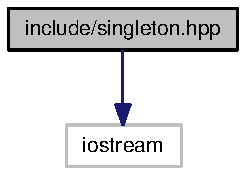
\includegraphics[width=77pt]{singleton_8hpp__incl}
\end{center}
\end{figure}
\subsection*{Classes}
\begin{CompactItemize}
\item 
class \hyperlink{classSingleton}{Singleton$<$ T $>$}
\begin{CompactList}\small\item\em Template de classe permettant de rendre une classe instanciable une seule fois. \item\end{CompactList}\end{CompactItemize}


\subsection{Detailed Description}
Implementation du design pattern singleton. 

\begin{Desc}
\item[Author:]GDD 

Arnaud Faure 

Pauline Requena \end{Desc}
\begin{Desc}
\item[Version:]0.1 \end{Desc}
\begin{Desc}
\item[Date:]29 mars 2009\end{Desc}
Implementation du design pattern singleton pour rendre une classe instanciable une unique fois. 
\hypertarget{table_8hpp}{
\section{trunk/include/table.hpp File Reference}
\label{table_8hpp}\index{trunk/include/table.hpp@{trunk/include/table.hpp}}
}
Implementation du module table qui est un derive d'un \hyperlink{classEcoAgent}{EcoAgent}.  


{\tt \#include $<$iostream$>$}\par
{\tt \#include \char`\"{}ecoAgentID.hpp\char`\"{}}\par
{\tt \#include \char`\"{}ecoAgent.hpp\char`\"{}}\par


Include dependency graph for table.hpp:

This graph shows which files directly or indirectly include this file:\subsection*{Classes}
\begin{CompactItemize}
\item 
class \hyperlink{classTable}{Table}
\begin{CompactList}\small\item\em Classe derivee de la classe \hyperlink{classEcoAgent}{EcoAgent} designant le support sur lequel vont etre poses les cubes. \item\end{CompactList}\end{CompactItemize}


\subsection{Detailed Description}
Implementation du module table qui est un derive d'un \hyperlink{classEcoAgent}{EcoAgent}. 

\begin{Desc}
\item[Author:]GDD 

Arnaud Faure 

Pauline Requena \end{Desc}
\begin{Desc}
\item[Version:]0.1 \end{Desc}
\begin{Desc}
\item[Date:]1er avril 2009\end{Desc}
Implementation de la classe \hyperlink{classTable}{Table} qui est une classe derivee de la classe \hyperlink{classEcoAgent}{EcoAgent}. La \hyperlink{classTable}{Table} est le support sur lequel sont poses les cubes. 
\printindex
\end{document}
